
\documentclass[12pt,oneside,letterpaper]{book}
%\usepackage[english, french]{babel}  %support francais et anglais
\usepackage[T1]{fontenc}
% Pour utiliser des fichiers UTF-8
%\usepackage[utf8]{inputenc}
\usepackage{lineno}
\usepackage{times}
\usepackage{mathptmx}
%\usepackage[pdftex]{thumbpdf}
\usepackage[table]{xcolor}% http://ctan.org/pkg/xcolor

\usepackage{xspace}

\usepackage{lscape}  %for the landscape table

\usepackage{threeparttable} %for footnotes within a table

\usepackage{dcolumn,amsmath}


\usepackage{udem_these_eng} %package pour une th�se de l'UdeM en Anglais
\usepackage{amsfonts}
\usepackage{amsthm}

\usepackage{epsfig}
\usepackage{float}

% Pour utiliser la fonte Computer Modern par defaut, commenter les
% deux lignes precedentes et decommenter la ligne suivante
%\usepackage{ae,aecompl,aeguill}
\usepackage{flafter}
\usepackage[pdffitwindow=false,
pdfview=FitH,
pdfstartview=FitH,
plainpages=false]{hyperref}

%to prevent errors from the colour

%\newcommand{\color}[2]{}

% Unique number for each line
%\linenumbers


% remplir les champs...

\Auteur{Christian }{Dansereau}

\President{M.}{Jean }{Meunier}{Ph.D.}

\Directeur{M.}{Pierre }{Bellec}{Ph.D.}

%omettre si il n'y a pas de codirecteur
%\CoDirecteur{M.}{Mauris}{ Proin}{Ph.D.}

\Membres{1}{M.}{Aaron }{Courville}{Ph.D.}

%pour le doctorat seulement
%examinateur externe
%\Membres{2}{Mme.}{Vel}{Venenatis}{Ph.D.}

%representant du doyen de la FES
%\Membres{3}{M.}{Mauris}{Erat}{Ph.D.}


%Pour un doctorat, changer simplement \MSc par \PhD
%titre: 15 mots, max. 175 caracteres

\PreDoc
{Selection of multiscale functional brain connections for early diagnosis of Alzheimer's disease in multicentric studies}
    {}
    {d'informatique et de recherche op\'{e}rationnelle}
   {computer science}
    {D�cembre}
    {2014}

% Cette commande definit \ell'espacement entre les lignes. Ceci permet
% de reduire le nombre de pages pour les version preliminaires.
% Pour la version finale, choisir entre 1.4 et 2, selon le gout.
\setstretch{1.4}
\begin{document}



\setcounter{page}{1}


\PagesCouverture

%\resume
\selectlanguage{french}


 %(150 a 250 mots) (1 page)

\noindent Donec luctus posuere ligula. Nunc rutrum mauris non
ligula. Cras dapibus. Etiam in sapien. Quisque vestibulum. Mauris
sodales malesuada velit. Curabitur vehicula. Morbi convallis, mi
ac tincidunt blandit, pede lacus mollis justo, sed mattis pede
ante ut odio. Integer euismod tincidunt ante. Pellentesque dolor
enim, commodo nec, vulputate et, semper sit amet, erat. Curabitur
quis velit.

Mauris convallis magna non lacus interdum facilisis. Praesent
purus. Nulla aliquam felis sed diam. Praesent nibh. Nulla
elementum blandit dolor. Ut tortor orci, tristique ut, vestibulum
eu, scelerisque sed, ipsum. Sed diam. Donec a dolor. In hendrerit,
mi sed hendrerit ornare, eros libero congue dolor, a iaculis lorem
ipsum nec nisl. Nullam velit libero, pharetra eu, ullamcorper ac,
posuere eu, odio. Class aptent taciti sociosqu ad litora torquent
per conubia nostra, per inceptos hymenaeos. Morbi sit amet est.
Nullam sed enim quis arcu adipiscing pretium. Fusce accumsan
commodo nulla. Nullam ipsum. Maecenas semper elit a nulla. Nullam
a magna eleifend libero convallis sagittis. Vivamus dui.

Vivamus nec magna sed mi faucibus convallis. Morbi et ipsum.
Maecenas scelerisque, erat eget molestie viverra, tortor turpis
pulvinar neque, sed pulvinar velit odio at tortor. Proin varius
feugiat purus. Sed dictum consequat wisi. Proin sit amet risus.
Pellentesque lectus. Ut sollicitudin justo ac nibh. Nulla felis.
Etiam pharetra. Duis vitae lectus.



{\bfseries Mots cl�s\hspace{-3pt}: Vivamus,  magna, sed, faucibus,
convallis.}


\selectlanguage{english}

\abstract

 %(150 a 250 mots) (1 page)
Functional magnetic resonance imaging (fMRI) gives a non-invasive measure of functional connectivity throughout the brain in individual human subjects. This imaging modality captures a massive amount of connections, in the order of $10^8$, some of which may be biomarkers of Alzheimer's disease (AD). The brain is highly structured into a nested hierarchy of networks, which can be leveraged to reduce the dimensionality of brain connectivity into a limited set of biologically meaningful features. The objective of this project is to develop multiscale clustering techniques for feature extraction, in conjunction with random forest for prediction of clinical diagnosis and prognosis of AD, using fMRI connectivity. I will investigate the case of multicentric fMRI data including a few hundreds of participants, i.e. the AD neuroimaging initiative (ADNI) sample, which is the typical design found in phase II pharmaceutical clinical trials. Site-specific MRI set-ups may bias the fMRI measures, and I am thus developing procedures for inter-site normalization. The main outcome of this project will be a prediction pipeline for the data-driven identification of AD biomarkers in resting-state fMRI.



%(max. of 10, not words in the title)
{\bfseries Keywords: fMRI, Alzeimer's disease, biomarker, multisite.}


\tabledesmatieres

\listedestableaux

\listedesfigures

%\listedesannexes

% \abbreviation
\begin{eqnarray*}
%\nonumber to remove numbering (before each equation)
% mettre en ordre alphabetique!!!!!!
 \text{DLR} & & \text{Duis Lacinia Rutrum } \\
  \text{NS} & & \text{Nullam Sagittis} \\
  \text{VRE} & & \text{Vestibulum Rutrum Elit }\\
\end{eqnarray*}

%\notation

\begin{center}
\begin{tabular}{r p{12cm} }
$\mathbb{R}$ & Ronec \\
$\mathbb{C}$ & Coretium   \\
$\imath$    & enim nec neque, $\imath = \sqrt{-1}$\\
 $|\alpha|$  & dapibus nonumly $\alpha$\\
 $\mathcal{H}_d$ & $d$-parturient montes \\



\end{tabular}
\end{center}

% \dedicace

  \vspace*{1.0cm}

   \hspace{2.5in}
    (dedicace) Cras semper lorem nec pede.

%\remerciements

Curabitur pharetra. Nam vestibulum ligula nec dolor. Donec ac
lectus. Integer eleifend mollis nunc. Phasellus at sapien eu velit
aliquam commodo. Cras vel erat non enim iaculis elementum. Etiam
non lacus sit amet arcu viverra fringilla. Aliquam blandit.
Quisque at odio. Nam vulputate elementum felis. Sed gravida. Sed
sem tellus, luctus commodo, pretium a, aliquam eu, enim.
Vestibulum ut neque vitae felis elementum porta. Suspendisse
potenti. Duis sed wisi. Nam accumsan, metus dictum scelerisque
nonummy, ipsum ipsum gravida arcu, nec viverra sem velit vitae
arcu. Suspendisse facilisis ante at leo. Vivamus nec libero
sagittis nunc hendrerit lacinia. Vestibulum ultrices vehicula
eros.

%\preface
Lorem ipsum dolor sit amet, consectetuer adipiscing elit. Nam
ipsum. Nulla vehicula diam non nisl. Curabitur rhoncus nulla ac
felis. Nam vel ipsum quis neque condimentum pretium. Maecenas ut
quam. Maecenas orci elit, feugiat sit amet, dignissim a, tristique
vel, ante. Proin sed turpis. Mauris pede. Phasellus congue felis
id odio. Maecenas lectus sapien, fringilla sed, elementum vitae,
posuere ut, mauris. Sed odio. Maecenas molestie. Curabitur ut nunc
id nulla lobortis facilisis. Sed blandit feugiat velit. Integer
arcu sapien, dapibus quis, adipiscing vitae, dignissim eget, pede.
Fusce tincidunt augue sed magna. Donec iaculis sagittis augue.


\debutchapitres
%%\introduction
\chapter{Introduction}

Lorem ipsum dolor sit amet (\cite{GHZ,EPR35}), consectetuer
adipiscing elit. Vestibulum id elit a magna aliquet viverra. Fusce
eleifend ultricies lectus. Duis luctus magna non elit. Fusce
risus. Aenean sodales viverra nibh. Nulla ac libero in nulla
vehicula pharetra. Praesent ac velit ac pede vestibulum
sollicitudin. Cras ipsum. Praesent dapibus blandit eros. Lorem
ipsum dolor sit amet, consectetuer adipiscing elit. Cras at dui.
Donec sagittis. Vivamus ut justo.

Phasellus \cite{Boojums} leo ligula, venenatis faucibus, malesuada
at, feugiat vitae, tortor. Donec magna tortor, egestas sit amet,
posuere id, elementum vel, nunc. Aliquam eleifend dictum quam.
Integer a quam. Vestibulum scelerisque, nulla eget interdum
pretium, ante leo egestas ligula, vel venenatis enim magna eget
nibh. Aenean in quam. Curabitur blandit dolor at dolor vestibulum
accumsan. Nullam turpis tortor, tristique laoreet, tempus vel,
mattis at, massa. Vestibulum ante ipsum primis in faucibus orci
luctus et ultrices posuere cubilia Curae; Vivamus blandit posuere
nunc. Maecenas bibendum pulvinar nunc. Vestibulum elementum felis
non orci.

Cras eget est Figure~\ref{fig:conditional}.

\begin{figure}
\begin{verbatim}
if
    (x>0)
then
    return x
else
    return -x;
\end{verbatim}
\caption{Morbi eu sem ac est porttitor viverra}
\label{fig:conditional}
\end{figure}


 Quisque id neque nec diam iaculis
rutrum.  Curabitur a urna suscipit erat accumsan tristique.
Maecenas nec lorem eget velit tincidunt congue. Morbi nulla justo,
blandit nec, semper non, suscipit eu, libero. In pellentesque leo.
In accumsan velit sed diam commodo vulputate. Lorem ipsum dolor
sit amet, consectetuer adipiscing elit. Quisque laoreet massa ac
tellus. Nam massa.

\section{Cum sociis natoque penatibus} \label{sec:introduction}

Curabitur eu nisl at risus vulputate tristique. In et lorem. In
suscipit porta dolor. Sed quis nulla quis justo bibendum iaculis.
Aenean nulla mi, accumsan at, luctus vel, sollicitudin non, odio.
Phasellus ac sem. Morbi ut neque et risus dictum tincidunt. Proin
at diam. Fusce nunc. Vestibulum in ipsum. Mauris hendrerit
suscipit risus. Maecenas in turpis sit amet enim tempus commodo.
Maecenas mattis libero vitae lorem.

Nulla facilisi. Curabitur wisi lorem, cursus id, nonummy non,
accumsan tristique, magna. Donec sit amet erat. Sed pretium dui at
justo. Nulla imperdiet. Maecenas vitae sapien. Nunc consectetuer
vestibulum felis. Cras laoreet, eros in accumsan bibendum, enim
augue feugiat arcu, a lobortis eros leo a augue. Cras ultricies
mauris at leo. Aliquam eu pede. Proin turpis.

Integer risus. Etiam congue, risus sit amet ornare molestie, orci
neque bibendum sapien, sed varius felis lacus eu felis. Praesent
condimentum mauris ac massa. Mauris vulputate feugiat risus.
Mauris euismod, nibh non varius molestie, tortor velit rhoncus
purus, nec mattis eros quam ut orci. Donec gravida ipsum sit amet
lacus. Mauris sodales, nunc vitae porttitor placerat, ipsum risus
viverra lectus, ut tempus nunc felis et orci. Vestibulum tortor.
Class aptent taciti sociosqu ad litora torquent per conubia
nostra, per inceptos hymenaeos. Integer turpis sapien, auctor sit
amet, ultricies posuere, sollicitudin eget, arcu. Vivamus faucibus
lorem nec mi. Sed egestas leo vel elit. Vivamus egestas, massa eu
viverra posuere, justo tellus commodo wisi, at faucibus elit justo
eu risus. Mauris fermentum, enim sit amet porta mattis, odio
sapien semper dui, rhoncus sodales est sem quis ligula. Vestibulum
vel odio sed ligula consectetuer accumsan. Fusce pulvinar mi ut
sapien. Phasellus at odio.

\section{Aenean magna risus}

Praesent est. Nulla at turpis. Vestibulum euismod urna quis
ligula. Integer consequat vulputate eros. Fusce sit amet ipsum.
Suspendisse lacinia sapien ac magna. Morbi lorem. Sed dictum nulla
eget purus. Nunc porta ante eu purus. Vivamus nec lacus ut leo
volutpat auctor. Phasellus auctor tincidunt mauris. Sed ultrices
ante venenatis arcu. Aenean mattis fringilla wisi. Aliquam nulla
lacus, pellentesque non, pretium non, vehicula a, enim. Nulla
sagittis. Nunc aliquet risus vel wisi sodales malesuada.
Pellentesque habitant morbi tristique senectus et netus et
malesuada fames ac turpis egestas.

\begin{table}[!ht]
\centering
\begin{tabular}{|c|c|}
  \hline
  % after \\: \hline or \cline{col1-col2} \cline{col3-col4} ...
 Praesent turpis sem& sodales\\
  \hline
  1 & a \\
  2 & b \\
  3 & c \\
  4 & d \\
  \hline
\end{tabular}
\caption{facilisis at libero}
\end{table}


Adipiscing sed, sodales in . Nam pharetra. Donec quam nisl,
adipiscing sit amet, rhoncus sit amet, varius in, quam. Fusce at
urna. Sed quis libero non dolor aliquet bibendum. Aliquam lacus
augue, auctor quis, congue eget, faucibus vitae, purus. Fusce
ullamcorper. Morbi consectetuer wisi quis velit. Nam purus justo,
feugiat et, iaculis et, imperdiet sit amet, risus. Suspendisse
tristique. Suspendisse non leo vitae orci adipiscing semper.
Vestibulum mauris urna, consequat eget, mattis a, ornare vitae,
enim. Phasellus tincidunt wisi in leo. Mauris sit amet nunc. Nam
eu wisi. Morbi tincidunt accumsan ipsum.



Praesent blandit pretium purus. Integer at velit sed sapien
ultricies pellentesque. Mauris et ligula sed odio dignissim
ornare. In non purus a tellus laoreet eleifend. Maecenas euismod
gravida turpis. Praesent hendrerit, erat a sollicitudin mollis,
metus mi feugiat ipsum, eu faucibus nulla magna id libero. Ut
adipiscing, nunc nec condimentum blandit, odio enim euismod
lectus, a gravida sem elit in metus. Ut ligula. Sed malesuada
lorem sed diam. Vivamus pharetra.



\chapter{General context}
The number of Canadians suffering from Alzheimer's disease (AD) is rapidly increasing, with tremendous social and economic impact. Despite the emergence of promising drugs, the recent clinical trials with demented patients have failed. Dementia however comes very late in the development of the disease, at a stage where the degeneration of neural tissues has likely gone beyond repair. In order to be efficient, therapies should be initiated in the decades predating dementia, in a preclinical stage where patients experience no or very mild symptoms (see chapter $1.1$). There are unfortunately no biomarker(s) that are currently predictive of AD in this preclinical stage, and could help identify the individuals that could benefit from such interventions. A promising technique is resting-state functional magnetic resonance imaging (rs-fMRI), which may be able to capture the early synaptic dysfunction seen in AD (see chapter $1.2$). I order to be able to apply statistical analysis and machine learning methods we 
need to preprocess the data to remove as much as possible the effect of various artefacts (hardware and physiological). The preprocessing reduces the variability of the data and therefore provides more relevant and discriminative features (see chapter $1.3$). In order to further improve the statistical power of there analysis, multiple academic groups are collaborating to pool their dataset to increase the sample size of the study. Unfortunately the gain in sample size comes with a new source of variability introduced by the multicentric acquisition. Site-specific MRI set-ups may bias the fMRI measures, and I am thus developing procedures for inter-site normalization. Account for these sources of variance are important since they may bias the predictive potential of rs-functional connectivity in a multi-site, in line with this last assumption we want to quantify the robustness of the feature selection and classifier to multi-site acquisition (see chapter $1.4$).

With the objective of extracting meaningful information that could be used as biomarkers we are using connectivity measures usually based on the correlation of spontaneous fluctuations in neurovascular activity from pairs of brain regions, which have been shown to be sensitive to the development of the disease (see chapter $1.5$). However, with about $10^4$ recording sites in the gray matter and close to no knowledge on the early brain dysfunction in AD, there is an overwhelming number of $10^7$ possible connections to examine as a potential diagnostic we will therefore focus on the feature selection procedure and the stability of those selections in order to have consistent and sparse predictive features discriminative of the disease(see chapter $1.6$). The main outcome of this project will be a prediction pipeline for the data-driven identification of AD biomarkers in resting-state fMRI.

\section{Alzheimer's disease} Alzheimer's disease (AD) is a major neurodegenerative disorder characterized by cognitive and intellectual deficits and behavioural changes without a known cause or an effective treatment. It gradually destroys a patient's memory and ability to reason, make judgments, communicate and carry out daily activities \citep{Jeong2004}. With the aging of the population worldwide, this disorder has attracted much attention. Evidence from clinical elderly individuals suggests that the pathophysiological process of AD begins years, if not decades, before the diagnosis of clinical dementia \citep{Morris2005}. The clinical disease stages of AD are divided into three phases described by Jack and colleagues \cite{Jack2010}. 

\textit{First is a pre-symptomatic phase in which individuals are cognitively normal but some have pathological changes in AD. Second is a prodromal phase of AD, commonly referred to as mild cognitive impairment (MCI) \citep{Petersen2004}, which is characterised by the 
onset of the earliest cognitive symptoms (typically deficits in episodic memory) that do not meet the criteria for dementia. The severity of cognitive impairment in the MCI phase of AD varies from early manifestation of memory dysfunction to more widespread dysfunction in other cognitive domains. The final phase in the evolution of AD is dementia, defined as multi-domain impairments that are severe enough to result in loss of function} \citep{Jack2010}.

The use of biomarker for the early diagnostic of pathologies has a long history, with many studies showing the feasibility of using AD biomarker to predict conversion from MCI to AD. These studies show that individuals on the course of developing AD can be identified earlier in the course of the disease by using the MCI stage with the addition of imaging and cerebrospinal fluid (CSF) biomarkers to enhance diagnostic specificity \citep{Chetelat2003,Jack1999,Yuan2009,Mattsson2009}. 
It could be possible to diagnose AD after the exclusion of other forms of dementia, although a formal diagnostic can only be made after a post-mortem evaluation of the brain tissue \citep{McKhann1984}. This is one of the reasons why MRI based analysis and diagnostic tools are currently a hot topic in clinical neuroscience research.

The currently dominant hypothesis in the field for the chain of events in AD pathophysiology is the $\beta$-amyloid (A$\beta$)-cascade hypothesis. It suggests that interstitial A$\beta$ proteins exert a toxic effect on surrounding neurons and synapses by forming plaques, thereby disturbing their function \citep{Hardy2002,Shankar2008}. Moreover, recent research study suggests that, prior to neuronal death resulting in brain atrophy, disruption of functional connectivity may arise in response to an unknown systemic problem and represent an early outcome of A$\beta$ proteins plaque formation in AD \citep{Sheline2013}. Atrophy is the result of neuronal death and is measures in vivo using structural MRI measuring the thickness of the gray matter on the cortex (also called cortical thickness). Already in the stage preceding aggregation of A$\beta$ fragments into amyloid plaques, there is a dysfunction of synaptic transmission in many brain regions due to dimers and monomers from the A$\beta$ cascade \citep{
dAmelio2012}. As illustrated in \cite{Sperling2011} a viable hypothesis is that fMRI precedes the structural changes as well as clinical symptoms and is believed to start in the preclinical phase of the disease.


\begin{figure}[H]
\begin{center}
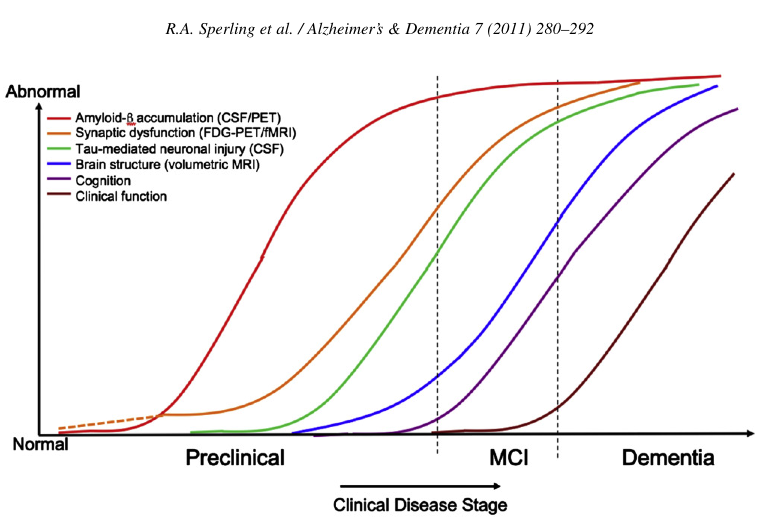
\includegraphics[width=\linewidth]{../figures/ad_progression.png}
\end{center}
\caption[Biomarker model of Alzeimer's disease]
{Hypothetical model of dynamic biomarkers of the AD expanded to explicate the preclinical phase: A$\beta$ as identified by cerebrospinal fluid A$\beta$42 assay or PET amyloid imaging. Synaptic dysfunction evidenced by fluorodeoxyglucose (F18) positron emission tomography (FDG-PET) or functional magnetic resonance imaging (fMRI), with a dashed line to indicate that synaptic dysfunction may be detectable in carriers of the 34 allele of the apolipoprotein E gene before detectable A$\beta$ deposition. Neuronal injury is evidenced by cerebrospinal fluid tau or phospho-tau, brain structure is evidenced by structural magnetic resonance imaging. Biomarkers change from normal to maximally abnormal (y-axis) as a function of disease stage (x-axis). The temporal trajectory of two key indicators used to stage the disease clinically, cognitive and behavioral measures, and clinical function are also illustrated. Figure from \cite{Sperling2011}.}
\label{fig_biomarker_model}
\end{figure}


\section{Overview of functional magnetic resonance imaging} In functional magnetic resonance imaging (fMRI), the acquisition process is slightly different than for the anatomical MRI acquisition. fMRI uses the principle of the relaxation of hydrogen nuclei, by using specific fMRI sequences consisting in $T2*$ weighted acquisitions that are sensitive to local distortions of the magnetic field. Particularly, deoxyhemoglobin (a form of hemoglobin without oxygen) will create such local distortions of the magnetic field, since it is a paramagnetic molecule (positive magnetic susceptibility) \citep{Ogawa1990}. The data acquired using fMRI rely on the hypothesis that areas showing decreased deoxyhemoglobin concentration are due to sustained brain activity. Following neuronal activity, neurons require energy to restore the electrical and ionic concentration balance across the cell membrane. One mechanism to generate this energy is the glucose oxidative metabolism, which requires the delivery of oxygen and glucose by 
the blood on the site where brain activity takes place \citep{Ogawa1990}
. Initially, fMRI was thought to be a good technique to measure the cerebral metabolic rate of oxygen, since the new blood rushing in causes a proportional effect on the venous-end, resulting in a decrease in deoxyhemoglobin concentration, and thus an increase in fMRI signal. The concentration of deoxyhemoglobin actually depends mainly on three factors or phenomena: metabolic rate of oxygen consumption, cerebral blood volume (CBV) and cerebral blood flow (CBF) \citep{Hoge1999}. As a result, the fMRI signal is the outcome of competing effects following neuronal activity
%. CBF augmentation tends to decrease the deoxyhemoglobin concentration due to an increase in the oxygenated blood (resulting in a increase fMRI signal). While an increase in cerebral metabolic rate of oxygen and CBV tends to increase deoxyhemoglobin within the tissue at the vicinity of the neural activity, resulting in a decrease fMRI signal due to the paramagnetic properties of deoxyhemoglobin. The fMRI signal is the result of competing effects 
 and fortunately these effects do not cancel out, allowing the detection of a net signal increase. We call the interrelation of theses effects the blood oxygenation level dependent (BOLD) effect.

\begin{figure}[H]
\begin{center}
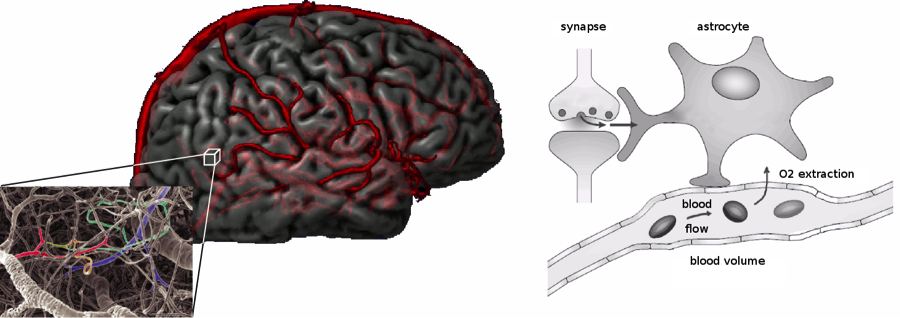
\includegraphics[width=\linewidth]{../figures/bold.png}
\end{center}
\caption[Schematic of the BOLD effect]
{Representation of the brain and its vasculature (on the left) and a schematic view of the interaction between the effect of neuronal activity on local changes in blood oxygenation signal (BOLD) (on the right) (adapted from \cite{Heeger2002}).}
\label{fig_bold}
\end{figure}

\section{Preprocessing}Normalization of the data is crucial to obtain a consistent and accurate classifier \citep{Kotsiantis2007}. Therefore a particular attention is place on the correction and normalization procedure applied to the rs-fMRI data used in this study. A series of standard preprocessing steps is usually applied in an attempt to correct for various artefacts that would perturb the subsequent analysis. The BOLD effect associated with neuronal activity generally results in a relatively small fluctuation of the MR signal. Many factors can influence this signal. Among them,  the physiological activity associated mainly with respiration, cardiac pulsations and patient's motion are major contributors to the noise and are spatially spread everywhere within the brain volume. These sources of noise result in large correlations between BOLD signals of distant voxels. An other factor is the fact that we need a form of spatial normalization of the individual brains in order to perform analysis across 
subjects (due to anatomical variance among subjects), this spatial normalization (coregistration of the individual brains with an reference template) is necessary but can potentially be an other source of confound. 
%Therefore, analyzing directly raw rs-fMRI data with seed-based connectivity or with a data driven technique (like ICA or clustering) will more likely result in the identification of noise related structures spread everywhere within the brain.
Therefore, preprocessing methods were designed in an attempt to remove specifically the so-called structured noise and motion artefacts from the raw fMRI data. A schematic representation of the preprocessing pipeline can be seen in Figure \ref{fig_preprocessing}.

\begin{figure}[H]
\begin{center}
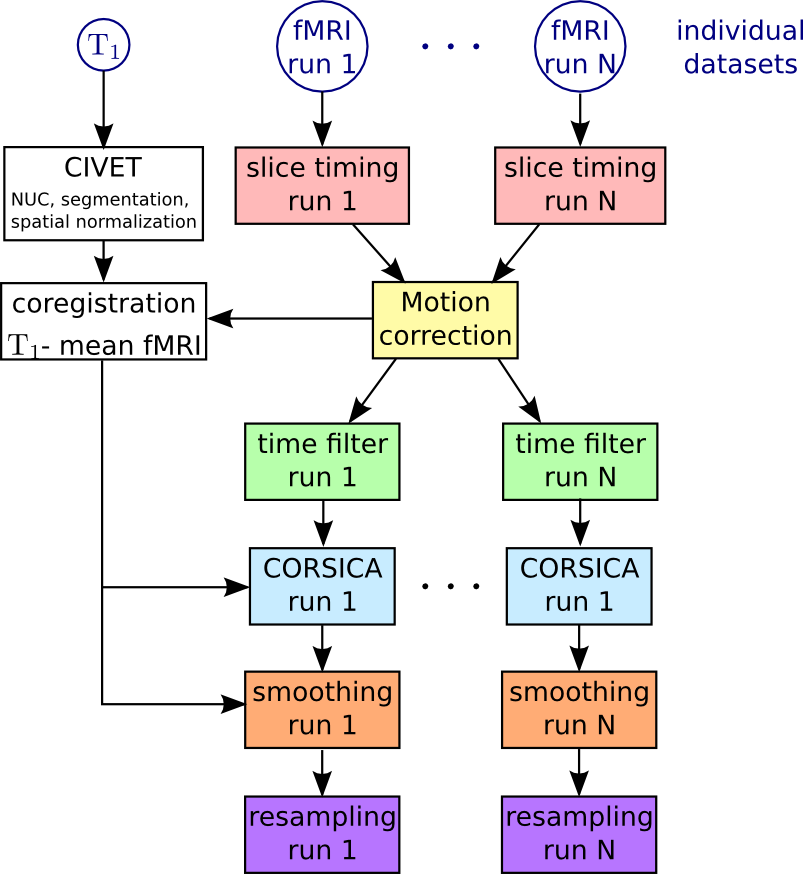
\includegraphics[scale=0.7]{../figures/fig_flowchart_fmri_preprocess.png}
\end{center}
\caption[Schematic of the preprocessing]
{Schematic of the preprocessing pipeline including spatial and functional normalization (NIAK preprocessing pipeline \footnote{\url{http://www.nitrc.org/projects/niak/}}).}
\label{fig_preprocessing}
\end{figure}

The basic steps are as follow: (1) correction for slice timing differences due to delay in acquisition sampling; (2) rigid-body motion estimation for within and between runs, motion correction operates by selecting one functional volume as a reference to align all other functional volumes. Most head motion algorithms describe head movement by 6 parameters, three translation (displacement) parameters and rotation parameters and are appropriate to characterize motion of rigid bodies (see Figure \ref{fig_motion_estimation}); (3) Coregistration of the functional data in a reference space; (4) resampling of the functional data in the stereotaxic space (references brain used as a common space between subjects); (5) regression of confounds in order to remove spatially structured noise on the fMRI 
time-series. The confounds are the slow time drift, high frequency noise signal, motion parameters, the average signal white matter as well as the average signal of the ventricles (containing cerebrospinal fluid CSF a frequent source of noise and artefact). Some groups have suggested that these corrections are not sufficient to remove motion artefact and propose some additional corrective procedure (detailed in Chapter 2); and (6) the spatial smoothing is usually applied using a Gaussian blurring kernel to improve signal to noise ratio (SNR), improved validity of the statistical tests by making the error distribution more normal and finally reduce anatomical and functional variations between subjects \citep{Worsley1995,Mikl2008}. %There is however a few drawbacks from this procedure like the reduction of spatial resolution of the data, edge artefact from smoothed brain voxels with non-brain voxels which might result in hypoactivation of the regions in question.

\begin{figure}[H]
\begin{center}
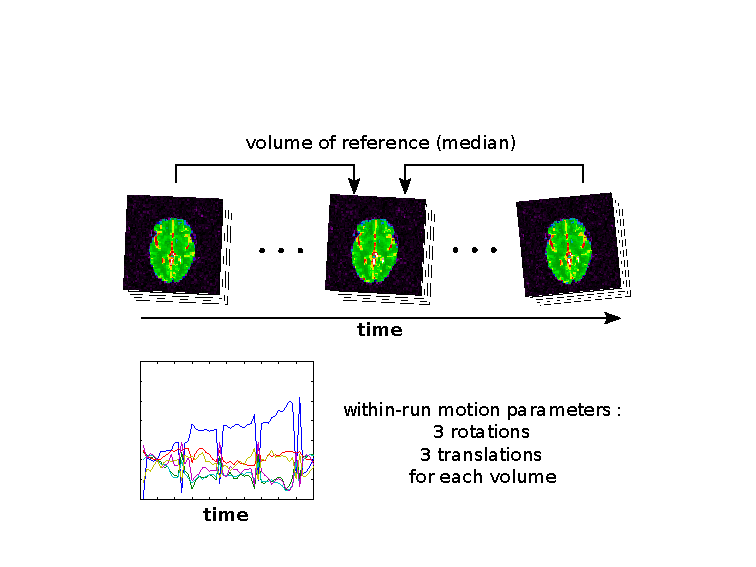
\includegraphics[scale=0.9]{../figures/motion_estimation.pdf}
\end{center}
\caption[Motion estimation]
{Motion estimation based on rigid-body motion estimation of the functional volumes, the procedure provide 6 motion parameters for each volume (3 translation and 3 rotation) Schematic of the preprocessing pipeline including spatial and functional normalization (from NIAK preprocessing pipeline \footnote{\url{http://www.nitrc.org/projects/niak/}}).}
\label{fig_motion_estimation}
\end{figure}



\section{Multi-site}
In most experiments conducted in neuroimaging, the main factors that influence power are: (1) the size of the effect, determined by the difference of the mean connectivity of one group versus a control group and the variability of this difference across subjects and groups; (2) the probability of rejecting the null hypothesis when it is true; and (3) the sample size, i.e. the number of subjects in the study \citep{Desmond2002}. This last factor is usually the only one controlled by the investigator, hence why an increasing number of researchers share multicentric, sometimes multiprotocol, data suitable to statistical analysis. In research it is very difficult to obtain a grant large enough to scan a cohort larger than ~80 subjects, therefore researcher and consortium initiatives have started to pool their resources together to make initiative composed of publicly available large cohorts of subjects like the 1000 functional connectome \citep{Biswal2010}, ADNI \citep{
Mueller2005}, among 
others. In clinical trial the justification for multicentric acquisition is more of a logistical one then a financial reason; they need to recruit a large amount of subject in a short period of time. In order to achieve this goal they mandate the recruitment to multiple clinical centers across the globe which accelerate the evaluation time of a drug. Although these centers may be similar by their scanner protocols, scanners will have difference in their software version, specific add-on to the scanners, and, most importantly, vendors (even field strength may differ in some cases). Unfortunately between studies, MR acquisition methodologies are among the most commonly cited sources of measurement variation \citep{Friedman2006}. This is why it is important to assess if multi-site resting-state connectivity analysis are feasible (we can combine the data from multiple sources while introducing a reasonable amount of variance which is still acceptable to detect effects in the data) and what corrective measure on 
the data should be applied to reduce the bias introduced by multi-site analysis. Among the factor of variability across sites, we can list the following 3 categories described in \citep{Yan2013a}:


\textit{
\begin{enumerate}
\item Acquisition-related variations:
\begin{enumerate}
\item Scanner make and model \citep{Friedman2006}
\item Sequence type (spiral vs. echo planar; single-echo vs. multi-echo) \citep{Klarhoefer2002}, parallel vs. conventional acquisition \citep{Feinberg2010} \citep{Lin2005}
\item Coil type (surface vs. volume, number of channels, orientation).
\item Acquisition parameters: repetition time, number of repetitions, flip angle, echo time, and acquisition volume (field of view, voxel size, slice thickness/gaps, slice prescription) \citep{Friedman2006a}.
\end{enumerate}
\item Experimental-related variations: 
\begin{enumerate}
\item Participant instructions \citep{Hartstra2011}, eyes-open/eyes-closed \citep{Yan2009} \citep{Yang2007}, visual displays, experiment duration \citep{Fang2007} \citep{VanDijk2010}.
\end{enumerate}
\item Environment-related variations: 
\begin{enumerate}
\item Sound attenuation measures \citep{Cho1998} \citep{Elliott1999}.
\item Attempts to improve participant comfort during scans (e.g., music, videos) \citep{Cullen2009}.
\item Head-motion restraint techniques (e.g., vacuum pad, foam pad, bite-bar, plaster cast head holder) \citep{Edward2000} \citep{Menon1997}.
\item Room temperature and moisture \citep{Vanhoutte2006}.
\end{enumerate}
\end{enumerate}
}


In 2009, the publicly released 1000 Functional Connectomes Project (FCP) and International Neuroimaging Data-sharing Initiative (INDI) provided a glimpse of the variability in imaging methodologies employed by the neuroimaging field. The dataset includes rs-fMRI samples independently collected at imaging sites around the world. A noteworthy aspect of this dataset is the variation in almost every parameter of the imaging acquisition methodologies, while the majority of subject-related variables are not reported (due in most cases, to the fact that they were not thoroughly recorded). 
Despite justifiable scepticism, feasibility analyses demonstrated that meaningful explorations of the aggregate dataset, composed of 24 imaging sites for a grand total of 1093 subjects, could be performed \citep{Biswal2010}. Although no explicit correction for multi-site variability was used, they only use global signal correction (GSC) to normalize subjects which may introduce anti-correlation in the data \citep{Fox2009, Murphy2009, Saad2012, Carbonell2014, Power2014}. After accounting for site-related differences, the analysis showed brain-behaviour relationships with phenotypic variables such as age, gender, and diagnostic label, and confirmed a variety of prior hypotheses \citep{Biswal2010, Fair2012, Tomasi2010, Zuo2012}. While encouraging, many uncontrolled and unknown factors in the 1000 FCP remain a source of concern, as they spread beyond simple site effects and can limit the datasets utility as highlighted by \cite{Yan2013}.
An other compelling proof of multi-site bias is the study reported by \cite{Nielsen2013} where they did an analysis on a single site dataset and a multi-site dataset of subject with autism and concluded that the multi-site autism study classification accuracy significantly outperformed chance but was much lower for multi-site prediction than for previous single site results \citep{Nielsen2013}. We therefore need to keep in mind that the site effect must be taken in account in the analysis or we may reduce our detection power.


\section{Resting-state connectivity}
Resting-state (RS) functional connectivity captures slow fluctuations of hemodynamic activity without performing any task. These temporal fluctuations can be monitored using the signal measured with fMRI. The first study that introduced the concept of resting state functional connectivity was the one of \cite{Biswal1995}. By performing a task activation response to bilateral left and right finger tapping, Biswal and colleagues were able to activate the corresponding motor areas on the cortex. In a second analysis, they considered one of the area activated during the task as a seed region for a seed-based analysis in resting-state condition. Seed-based analysis consists in detecting temporal correlation between the signal of the predefined seed area and the time course of all the voxels of the brain. Using this seed-based analysis, they found RS correlations between similar brain regions than the ones involved during the task. A more recent review done 
by \cite{Fox2007} illustrated in Figure \ref{fig_rs} show the ability to identify the complete sensorimotor network using only the bold signal from a small region in that network. 

\begin{figure}[H]
\begin{center}
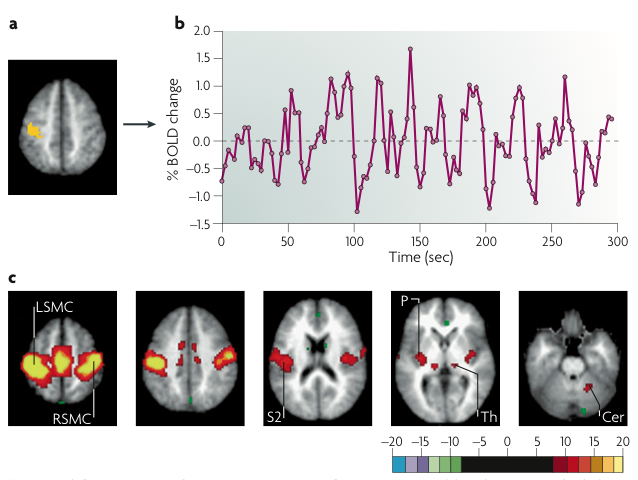
\includegraphics[width=\linewidth]{../figures/resting_state.png}
\end{center}
\caption[Resting-state correlation maps]
{Generation of resting-state correlation maps. a) Seed region in the left somatomotor cortex (LSMC) is shown in yellow. b) Time course of spontaneous blood oxygen level dependent (BOLD) activity recorded during resting fixation and extracted from the seed region. c) Statistical z-score map showing voxels that are significantly correlated with the extracted time course. Their significance was assessed using a random effects analysis across a population of ten subjects. In addition to correlations with the right somatomotor cortex (RSMC) and medial motor areas, correlations are observed with the secondary somatosensory association cortex (S2), the posterior nuclei of the thalamus (Th), putamen (P) and cerebellum (Cer) \citep{Fox2007}.}
\label{fig_rs}
\end{figure}

In resting-state acquisition, no task is performed during the scan; the subject is instructed to rest with his eyes open or closed, as opposed to the task-based acquisition where the subject has to perform a specific task. These early results from Biswal et al. suggest that it is possible to identify the functional organization of different structures without doing any specific task, just by looking at spontaneous fluctuations in brain activity. Several studies have demonstrated that patterns extracted from temporal correlations of rs-signals within the brain volume are organized in space and have a good reproducibility from subject to subject: the so-called consistent resting state networks (CRSN) \citep{Damoiseaux2006}. Each network is a combination of multiple brain regions or units, not necessarily spatially close to each other, which are sharing similar low frequency fluctuations of the BOLD signal; this is usually represented as a functional connectivity matrix where one column of the matrix represent 
the connectivity of a region with the rest of the brain called a 
functional connectivity map (see Figure \ref{fig_connectome} for a graphical representation of the two concepts).


\begin{figure}[H]
\begin{center}
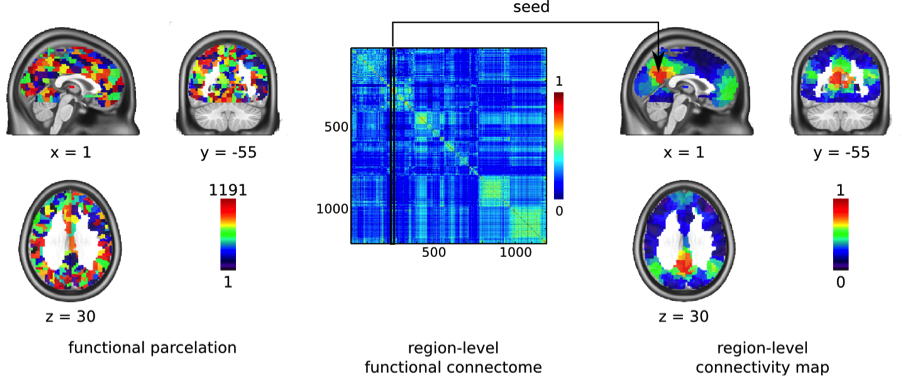
\includegraphics[width=\linewidth]{../figures/connectome.png}
\end{center}
\caption[Functional connectome]
{Functional connectome: on the left a representation of a functional parcellation, in the middle a region-level functional connectome representing the connectivity between each pair of region and on the right the connectivity map based on a region of interest extracted from the functional connectome.}
\label{fig_connectome}
\end{figure}

Several techniques have been used to identify these so-called resting-state networks (RSN). These networks show the functional organisation of various brain regions and several studies have demonstrated the relation of those functional networks to specific tasks in humans as well as in animal models \citep{Biswal1995} \citep{Buckner2008} \citep{Greicius2009}. Cordes et al. describe that several functional networks (sensorimotor, language and visual) identified in RS condition were exhibiting similar regions than the ones involved when performing a specific task (motor, language, or visual task) \citep{Cordes2000}. Based on such observations, CRSNs were then labeled according to the corresponding brain areas found active when performing such a specific task (e.g. motor or cognitive for example) thus associated with a brain function: e.g. auditory, visual, language networks \citep{Cordes2000} see Figure \ref{fig_crsn} for a list of common RSN. It enables us to establish the relationship between regions active 
when 
performing a specific task and RSNs, thus supporting the functional relevance of these networks. 


\begin{figure}[H]
\begin{center}
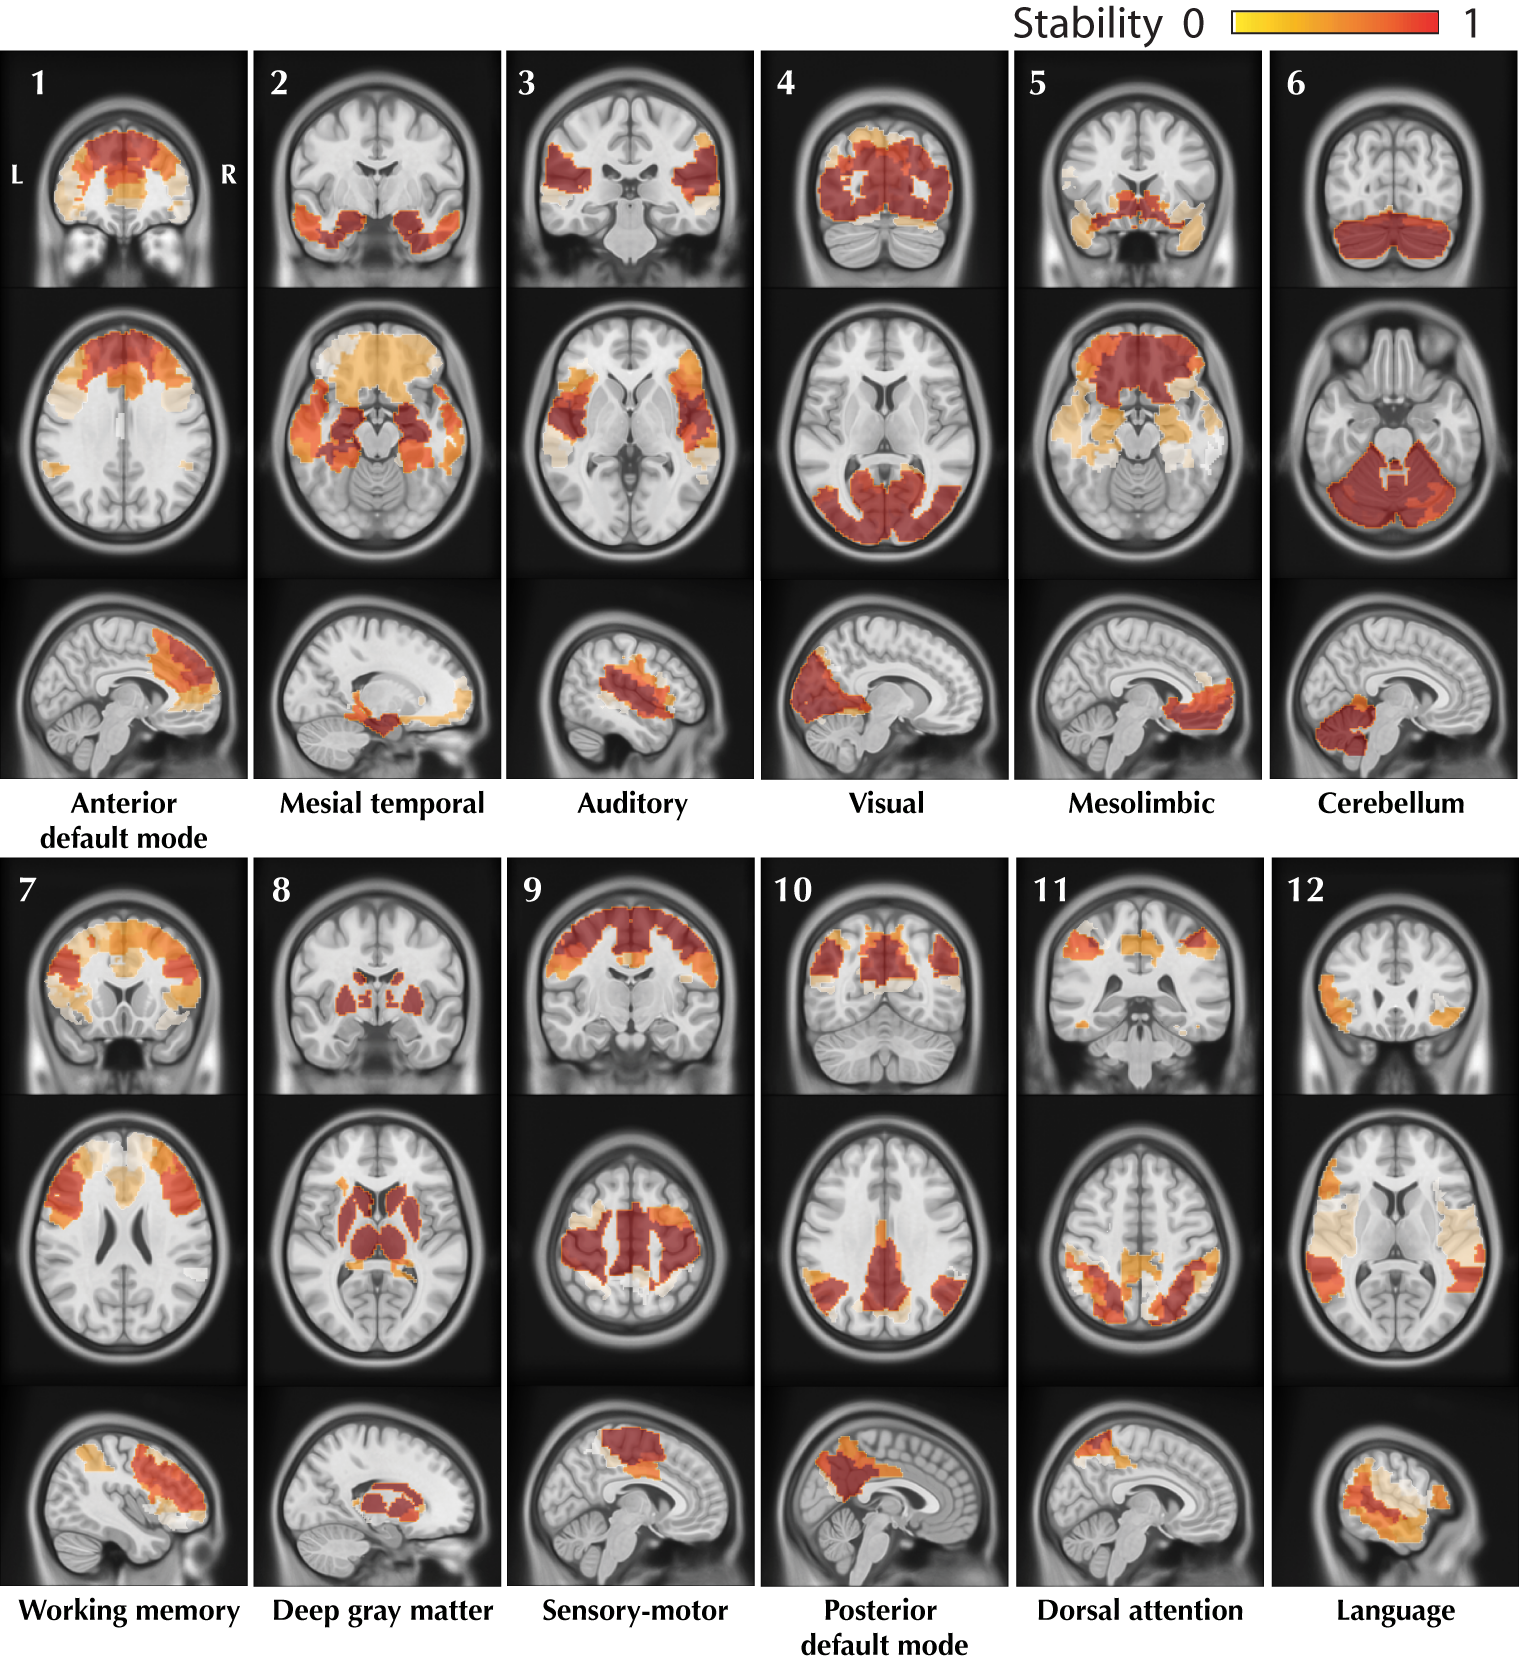
\includegraphics[scale=0.40]{../figures/CRSN.png}
\end{center}
\caption[Consistent resting-state network (CRSN)]
{The figure shows 12 CRSNs identified using BASC (Bootstrap Analysis of Stable Cluster \citep{Bellec2010c}) group level
analysis of 25 healthy control subjects. BASC is a clustering based method using evidence accumulation for the identification of stable cluster. For each CRSN: 3 slices (coronal, axial, sagittal)
are shown superimposed on an anatomical MRI template (MNI152). Labelling of each network was done visually based on previously reported CRSNs in the literature. The figure shows the usual networks: Default Mode Nettwork (\#1,\#10), Auditory (\#3), Visual (\#4), Sensory-Motor (\#9), Attention (\#7,\#11) and Language(\#12). BASC also identified 4 other networks, less often reported, but characterized by high statistical stability: Mesio-Temporal (\#2), Mesolimbic (\#5), Cerebellum (\#6) and Deep Gray Matter (\#8) \citep{Dansereau2014b} in press.}
\label{fig_crsn}
\end{figure}

Subsequently, rs-fMRI signal have been used in healthy subjects to investigate normal brain function, within various functional systems, such as auditory \citep{Cordes2001}, visual \citep{Lowe1998}, language \citep{Hampson2002}, limbic systems \citep{Greicius2003, Tian2007, Wink2006} and motor \citep{Jiang2004, Lowe1998}. Interestingly, resting-state fMRI signals have also been used to characterize the pathophysiological changes of some diseases, such as multiple sclerosis \citep{Lowe2002}, epilepsy \citep{Waites2006}, schizophrenia \citep{Liang2006, Salvador2007, Zhou2007, Zhou2008}, attention deficit hyperactivity disorder \citep{Tian2007, Zang2007}, blindness \citep{Liu2007, Yu2007}, major depression \citep{Anand2005, Greicius2007} and acute brainstem ischemia \citep{Salvador2005}. Thus, we believe that resting-state fMRI will be an increasingly important modality for exploring the functional abnormalities of patients with AD. Since a clinically meaningful hierarchical structure exist in the brain it is 
possible to use this structure to reduce the dimensionality of the problem and variability of the data while providing an informed organisation of the structure to a machine learning procedure looking to find functional markers characteristic of specific pathological populations (e.g. Alzheimer's disease).



\section{Prediction}
\subsection{Prediction in the context of AD}
In the past few years, several major studies have been initiated that have aimed to predict who will develop AD at the prodromal or even asymptomatic stage, with the ultimate goal of providing a platform for therapeutic intervention with disease-modifying therapies. Many of these studies were designed to evaluate the role of neuroimaging and chemical biomarkers in assessing and predicting progression in individuals without cognitive impairment and in individuals with MCI.
A very small literature currently reports findings on AD using rs-fMRI and they usually have outstanding performance like \citep{Jiang2014} ($94\%$). Unfortunately, the authors of this study performed a 10-fold cross-validation which did not include the feature selection process, which potentially lead to overestimation of the real accuracy. The rest of published studies have mainly used leave one out cross-validation and small sample size, which raises some concern with regards to the generalization ability of those trained predictors, e.g. \citep{Chen2011} ($87\%$), \citep{Dai2014} ($80\%$)).

\subsection{Importance of preprocessing to improve classification}
Preprocessing and normalization of the source data is a crucial point that may affect greatly the resulting classification or potential outcome measures. Moreover the introduction of multicentric data in the classification will render the task even more difficult, Nevertheless, a multi-site cohort helps test generalizability of the results across different samples, making it more likely that connections identified as predictive of a disease state indeed reflect generic traits of the pathology rather than particularities of a single dataset.

\subsection{High dimensionality problem}
In rs-fMRI, we obtain signal from brain activity at the voxel level representing more than $10^4$ voxels in the gray matter cortex, where the vast majority of the neurons are located. Although preprocessed, these data continue to have a lot of variance and we need to identify functional organisation more meaningful in term of clinical interpretation as well as an improved representation of the feature space that enhance the characterization of the functional modules. We can commonly extract functionally and clinically meaningful network features using principal component analysis (PCA) \citep{Zhong2009}, independent component analysis (ICA) \citep{McKeown1998}, various clustering algorithms such as k-means \citep{Baumgartner1998}, hierarchical clustering \citep{Cordes2002}, normalized cut-graph \citep{Heuvel2008}, self-organizing maps and neural gas \citep{Meyer-Baese2004}. Once we have functional parcels 
of the brain it is important to find the right metric to evaluate the connectivity between regions of the brain at the individual level. The most common metric use in the field of connectivity is the Pearson's correlation coefficient between the time series associated with a pair of regions.

\subsection{Feature selection}
Feature selection is often a critical step prior to any learning algorithm. The selection reduces the computational complexity of learning algorithms and exposes potentially clinically meaningful information. In many cases, this process can also improve the prediction accuracy by removing redundant and irrelevant information. Therefore feature selection is an important step in effective learning of large data sets. The features selection methods are usually organized into two categories: filter methods and wrapper methods \citep{Kotsiantis2007}. The filter method evaluates the relevance of features by looking only at the properties of the data without any knowledge on the classification labels. The wrapper method assesses the goodness a feature subset using the performance of a learning algorithm. The lack of reproducibility of reported markers (subset of features) is one of the main obstacle for the adoption of such marker in a clinical setup. If the marker is 
indeed discriminative of the pathology or of its progression we would expect the same features to be selected and exhibit similar performance across various studies. 

%relief proposed by xx is a feature selection method who try to optimise the margin between to class by selecting a sub sample of the features. An other algorithm called SIMBA proposed by algorithm proposed by Gilad-bachrach and colleagues in 2004 called margin based feature selection that aim to find the subset of features maximizing the margin between two classes.
%ensemble-based method \citep{Polikar2006} like Ada-boost to combine multiple week learners together

\subsection{Classification}
Machine learning methods have become very popular to classify functional brain images \citep{Costafreda2009,Fu2008,Hahn2011,Marquand2008,Nouretdinov2011}, for example to discriminate them between healthy and diseased populations. The most popular machine learning techniques in fMRI arguably is support vector machine (SVM) \citep{Cortes1995} which has been used in the past to categorize individual structural or functional brain images by differentiation of images from two groups (e.g. patient/control or male/female) \citep{Lao2004, Fan2005, Mourao-Miranda2005, Kawasaki2007}. 
%There is a modified version of SVM proposed by \cite{Li2011} called ccSVM who modify the kernel in order to account for confounding effects. 
A second widely used method is linear discriminant analysis (LDA) classifier; the main advantage of LDA is the ability to easily include confounding effects in the decision model, such as the inter-site difference in average connectivity measures.

\section{Objectives}
The objectives of the theses is to 1) reduce motion-related bias in connectivity measures, 2) evaluate the feasibility of multicentric fMRI analysis as well as identifying normalization procedures to reduce the between-site variance, and 3) design a prediction pipeline for the data-driven identification of biomarkers of AD in resting-state fMRI. The pipeline will have a feature selection tool to find a highly reduced set of functional connections with good prediction accuracy for the future conversion to a dementia of the Alzheimer's type in individuals with mild cognitive impairment.

\chapter{Scrubbing and motion artefact correction} 

\section{Introduction} Head motion is probably the most severe problem in fMRI studies, although it cannot be avoided. The quality of the fMRI data is strongly affected by the presence of head motion. As previously mention, a number of publications have proposed post-hoc correction in order to reduce head motion artefact. Although head motion can be corrected in the image space, displacement of the head reduces the homogeneity of the magnetic field, which is fine-tuned prior to functional scans for a given head position. Since head displacements lead to non-optimal tuning, motion artefacts are not fully removed even after perfect realignment of successive functional volumes in image space. The impact of motion and the method available to reduce its effect on functional connectivity thus need to be carefully evaluated. Typically subjects with average motion over 3 mm are excluded from the analysis. A first popular technique to reduce motion artifact is global signal correction (GSC), which consists of 
regressing the average of all the time-series in the brain. This 
technique has raised a number of concerns due to the potential artificial introduction of anti-correlation in the data \citep{Fox2009,Murphy2009, Saad2012, Carbonell2014, Power2014}. Another corrective measure is the CompCor method \citep{Behzadi2007} that regresses out the $n$ first components of a principal component analysis (PCA) on the time-series of the white matter and cerebrospinal fluids voxels. As no signal of neuronal origin are expected in such areas, the CompCor method was suggested to provide a compact representation of the structured noise present in an fMRI dataset. Both GSC and CompCor are global corrections, which are not specific to motion correction. The GSC in particular incorporates signal from the grey matter regions. Power and colleagues showed in 2012 that spurious but systematic correlations in fc-MRI arise from subject motion even at levels previously regarded as insignificant  (variation smaller than $1$ mm / degree in motion parameters) and are not adequately removed by common 
functional connectivity processing steps. \cite{Power2012} suggested using a method called ``scrubbing'' (or censoring) in order to reduce motion-related bias from  fMRI time-series. With the scrubbing method, the frames with motion level above a certain threshold are simply removed from the time-series. The metric used to quantify the level of motion from one frame to the other is called framewise displacement (FD). It is calculated as the sum of the absolute values of the differentiated realignment parameters estimated at every time point, giving an approximate conversion of rotation parameters ($\alpha_{i},\beta_{i},\gamma_{i}$) in a unit equivalent to a translation in millimeters on a sphere of radius 50mm and translation parameters ($d_{ix},d_{iy},d_{iz}$) for the other rigid body parameters.
The main limitation of the scrubbing method is the loss of time-points, which can lead to subjects loss due to an insufficient number of time point remaining after scrubbing correction. The question is therefore to evaluate if the trade-off between data loss and quality is detrimental or beneficial to statistical power. I have recently published results concerning this issue \cite{Dansereau2014} (published proceeding and manuscript in preparation). In this work we aimed to (1) characterize the impact of motion on rs-fMRI in cognitively normal elderly (CNE)  participants as well as patients with mild cognitive impairment (pMCI) and dementia of the Alzheimer's type 0.5-No (pDAT), and, (2) evaluate how the scrubbing impacts the differences in connectivity between groups (CNE, pMCI, pDAT).

\begin{equation}\label{Frame displacement} 
  \triangle d_{ix} = d_{(i-1)x} - d_{ix}\text{, derivative of a translation parameter in the x axis}
\end{equation}

\begin{equation}\label{Frame displacement}  
    FD_{i} = \vert \triangle d_{ix} \vert + \vert \triangle d_{iy} \vert + \vert \triangle d_{iz} \vert + \vert \triangle \alpha_{i} \vert + \vert \triangle \beta_{i} \vert + \vert \triangle \gamma_{i} \vert.  
\end{equation}

\section{Method}
\subsection{Dataset}
This project was based on a real dataset with fMRI data acuquired in different settings. The dataset included 313 elderly adults agregated across 5 independent studies: the ADNI2 study and 4 other studies based in Montreal, Canada. The dataset included three different clinical cohorts, for a grand total of 126 CNE participants (51 males, age range = 57-94 yrs), 133 patients with MCI (70 males, age range = 55-89 yrs), and 54 patients with DAT (22 males, age range = 55-88 yrs). We also included 355 cognitively normal young adults (CNY) from the 1000 functional connectome project (150 males, age range = 18-46 yrs) as a reference dataset \citep{Biswal2010}. This project was approved by the local ethics review board. 

\subsection{Preprocessing}
The datasets were analysed using the NeuroImaging Analysis Kit (NIAK\footnote{\url{http://www.nitrc.org/projects/niak/}}) version 0.12.14, under CentOS version 6.3 with Octave\footnote{\url{http://gnu.octave.org}} version 3.8.1 and the Minc toolkit\footnote{\url{http://www.bic.mni.mcgill.ca/ServicesSoftware/ServicesSoftwareMincToolKit}} version 0.3.18. Analyses were executed in parallel on the "Mammouth" supercomputer\footnote{\url{http://www.calculquebec.ca/index.php/en/resources/compute-servers/mammouth-parallele-ii}}, using the pipeline system for Octave and Matlab \citep{Bellec2012}, version 1.0.2. Brain map visualizations were created using MRICron software \citep{Rorden2007}. Each fMRI dataset was corrected of inter-slice difference in acquisition time and the parameters of a rigid-body motion was estimated for each time frame. Rigid-body motion was estimated within as well as between runs, using the median volume of the first run as a target. The median volume of one selected fMRI run for each subject 
was coregistered with a T1 individual scan using Minctracc \citep{Collins1998}, which was itself non-linearly transformed to the Montreal Neurological Institute (MNI) template \citep{Fonov2011} using the CIVET pipeline \citep{Zijdenbos2002}. The MNI symmetric template was generated from the ICBM152 sample of 152 young adults, after 40 iterations of non-linear coregistration. The rigid-body transform, fMRI-to-T1 transform and T1-to-stereotaxic transform were all combined, and the functional volumes were resampled in the MNI space at a 3 mm isotropic resolution. The 'scrubbing' method of \citep{Power2012}, was used to remove the volumes with excessive motion with three cut-offs points: no scrubbing ($FD\geq0$), $FD\geq0.5$ and $FD\geq0.2$. A minimum number of 50 unscrubbed volumes per run, corresponding to $\sim 125$ s of acquisition for a TR of 2.5 seconds, was then required for further analysis. For this reason, some subjects were rejected from the subsequent analyses: 11 CNE, 13 pMCI 
and 3 pDAT for a scrubbing at $FD\geq0.5$ and 83 CNE 95 pMCI and 39 pDAT for a scrubbing at $FD\geq0.2$ (see table \ref{tab_retention}). The following nuisance parameters were regressed out from the time series at each voxel: slow time drifts (basis of discrete cosines with a 0.01 Hz high-pass cut-off), average signals in conservative masks of the white matter and the lateral ventricles as well as the first principal components (95\% energy) of the six rigid-body motion parameters and their squares \citep{Lund2006},\citep{Giove2009}. The fMRI volumes were finally spatially smoothed with a 6 mm isotropic Gaussian blurring kernel. 

\subsection{Statistical analysis}
Impact of motion and scrubbing level on connectivity was estimated with a $t$-test and a group false-discovery rate (FDR) \citep{Hu2010}. Group differences (CNE, pMCI and pDAT) were investigated using $t$-tests for ten point-to-point 
connections selected based on a literature review \citep{Dansereau2013} including covariates to model age, gender and site-specific bias using model averaging \citep{Willer2010}. The significance of the difference in average connectivity between the clinical cohorts was assessed by a $t$-test in a linear model, including covariates to model site-specific bias. This procedure lead to a $p$-value estimating the false positive rate when testing against the null hypothesis of no group difference. To test the robustness of the group differences, the $t$-tests ($p\leq0.05$) were replicated $B=10^4$ times using random subsamples including $70\%$ of each group. For each replication $b$, a $p$-value $p^{*b}$ was generated. The stability of detection of a group difference as significant was estimated by the following Monte-Carlo average: 
\begin{equation}\label{Detection power}  
    B^{-1}\sum\limits_{b=1}^B\left(p^{*b}\leq0.05\right).
\end{equation}

\section{Results} 
\subsection{Motion distribution in different clinical cohorts}
A wide range of motion level was observed in the sample (Figure \ref{fig_dist}) and over all the elderly population seams to have more motion than the CNY. Even when scrubbing aggressively the difference in FD distribution between groups remained. We therefore needed to account for FD differences in subsequent analysis. In Figure \ref{fig_dist} a good overlap in the FD distribution across groups has been observed, the effect of scrubbing reduce the spread of the distribution and center the average FD around 0.2 (for scrubbing with a threshold $FD\geq0.5$) and 0.1 (for a threshold of $FD\geq0.2$). Overall the ammount of motion observed in CNY subjects was smaller than the one observed in the elderly populations (ECN, pMCI, pDAT) as shown in the boxplot representation on the left of Figure \ref{fig_dist}. In all preprocessing strategies the CNY remain significantly different in terms of FD compared to all the elderly groups. In term of the comparisons in FD distribution between elderly cohorts, scrubbing was 
able to remove some of the variability between groups but not 
sufficiently to remove the significant differences in FD in the CNE minus pMCI and CNE minus pDAT comparisons. The differences between pMCI and pDAT were not significant regardless of the preprocessing strategy. Surprisingly, results also showed that in the elderly population, the pDAT population was the one with the smallest amount of motion, followed by pMCI and finally CNE. There was no indication that the motion artifacts (and corresponding data quality) would be inferior in clinical populations. The is a 
significant difference in FD distribution between CNY and all the other groups in the 3 preprocessing strategies (see Figure \ref{fig_dist} on the right). Significant differences in term of FD distribution arose when scrubbing at $FD\geq0.5$ and $FD\geq0.2$ between the pDAT group and pMCI as well as pDAT and CNE group.
\par
Regarding the impact of scrubbing on the retention of the original dataset, 90\% of subjects survived the exclusion criteria of a minimum of 50 frames after scrubbing at $FD\geq0.5$ and 30\% survived an aggressive scrubbing of $FD\geq0.2$, see Table \ref{tab_retention} for the specific breakdown by clincal cohorts of elderly subjects (CNE, pMCI and pDAT). Only 1\% of the subjects were lost in the CNY cohort (99\% retention) for an $FD\geq0.5$ and 65\% survived for $FD\geq0.2$.

\begin{table}[H]
\begin{center}
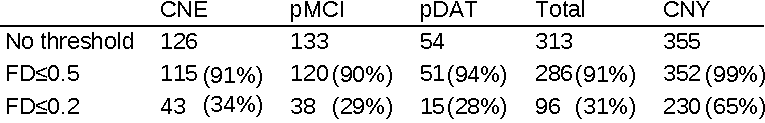
\includegraphics[width=0.75\linewidth]{../figures/table_retention.pdf}
\end{center}
\caption[Retention table after scrubbing]{
Retention rate for CNY, CNE, pMCI and pDAT at various scrubbing levels (standard, scrubbing $FD>0.5$ and scrubbing $FD >0.2$).
}
\label{tab_retention}
\end{table}

\begin{figure}[H]
\begin{center}
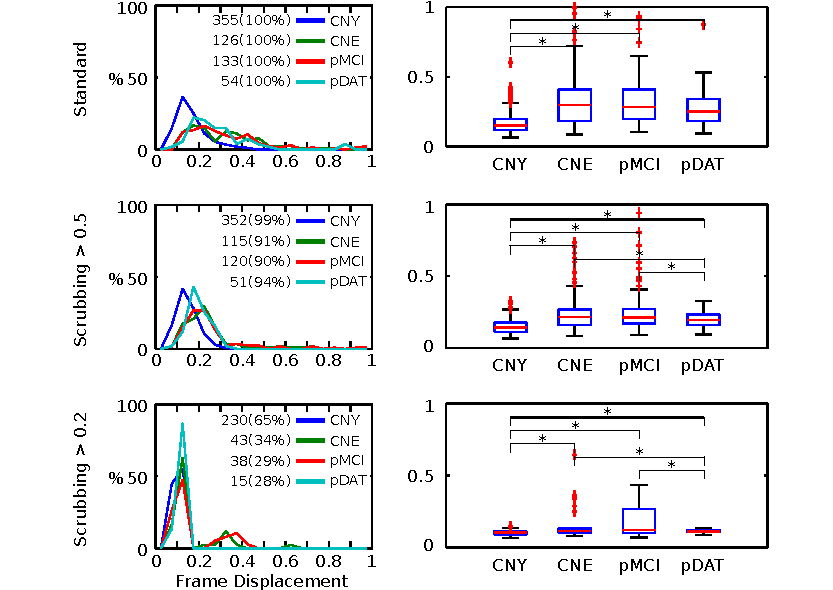
\includegraphics[width=\linewidth]{../figures/figure_fd_distrib.pdf}
\end{center}
\caption[FD distribution among groups]{
Distribution of the frame displacement (FD) for 3 groups (CNE, pMCI, pDAT) when scrubbing was applied at various levels (no scrubbing, scrubbing of $FD>0.5$ and scrubbing of $FD>0.2$). The boxplot on the right showed the distribution of FD with their associated statistical differences $t$-test (marked with a {\bf *} for a $p<0.05$).
}
\label{fig_dist}
\end{figure}

\subsection{Default mode network in young adult and elderly population}
The default-mode network (DMN) is hypothesized to be a key target of neurodegeneration in Alzheimer's disease. A visual inspection of the DMN using a standard preprocessing strategy showed more positive correlation values in the CNE population compared to the CNY (See Figure \ref{fig_avg_dmn}), probably reflecting increased partial-volume effect with cerebro-spinal fluids due to the large amount of cortical atrophy typically seen in aging. Moreover, a slight decrease in connectivity was observed in the frontal part of the DMN in the CNE population compared to the more common pattern of fronto parietal connectivity shown in the CNY population. This finding of more negative correlation for CNE subjects compared to CNY subjects was consistently observed regardless of the preprocessing strategies except for GSC, see Figure \ref{fig_avg_dmn}. The GSC seemed to increase the extent of the negative correlation found in other preprocessing strategies, as previously reported in the literature, e.g. \citep{Murphy2009}.


\begin{figure}[H]
\begin{center}
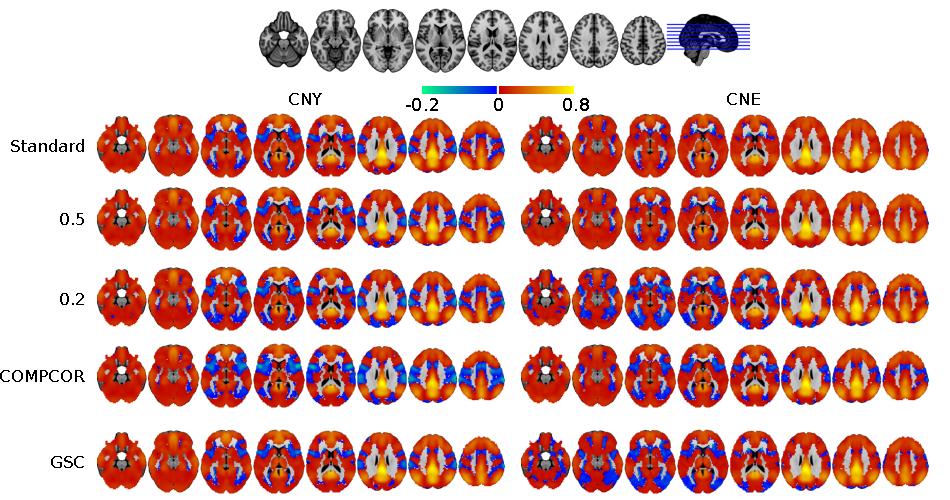
\includegraphics[width=\linewidth]{../figures/dmn_cny_cne.pdf}
\end{center}
\caption[Preprocessing impact on DMN for CNY and CNE]{ Overlay of the average default mode network (DMN) with various preprocessing strategies for CNY and CNE populations on the ICBM 152 anatomical atlas. Seed based maps with a seed in the PCC using Fisher z transform of the Pearson's r correlation between the average time series of each network.
}
\label{fig_avg_dmn}
\end{figure}

The connectivity patterns affected by scrubbing are consistent across various groups with and without dementia see Figure \ref{fig_scrubbimpact} for an example of three groups. The scrubbing procedure significantly increased connectivity strength inside the default-mode network and reduced connectivity with anti-correlated regions (Figure  \ref{fig_scrubbimpact}) consistently across all groups. More global decrease in connectivity changes can be observed for the CompCor and GSC methods. For CompCor a strong change in the sensory motor network can be observed as well as an increased connectivity in the ventral part mesio-frontal cortex. For the GSC method decreases in connectivity can be observed across the brain as well as a strong decrease in the occipital lobe.


\subsection{Impact of scrubbing on the connectivity}
\paragraph{Global impact of scrubbing}
Scrubbing significantly increased connectivity strength inside the default-mode network and reduced connectivity with anti correlated regions. Difference in functional connectivity of the DMN show significant increase of the frontal part of the DMN with scrubbing at $FD\geq0.5$ and $FD\geq0.2$ a region normally positively correlated with the PCC (see \ref{fig_scrubbimpact}). Significant decrease of connectivity with region associated with attention are also observed (dorsal attention network). The preprocessing with CompCor show massive decrease in the sensorimotor region and globally across the brain except for a mesio frontal region (anterior cingulate cortex ACC) more ventral then the expected mesio frontal region associated with the DMN (medial prefrontal cortex MPFC). The map of difference for the GSC show massive decrease in connectivity across the brain and in particular the occipital lobe, premotor and sensorimotor areas. The effect reported for the preprocessing with GSC are even more pronounced for 
the CNY group (see supplementary material Figure \ref{fig_sup_scrubbimpact_cny}).


\begin{figure}[H]
\begin{center}
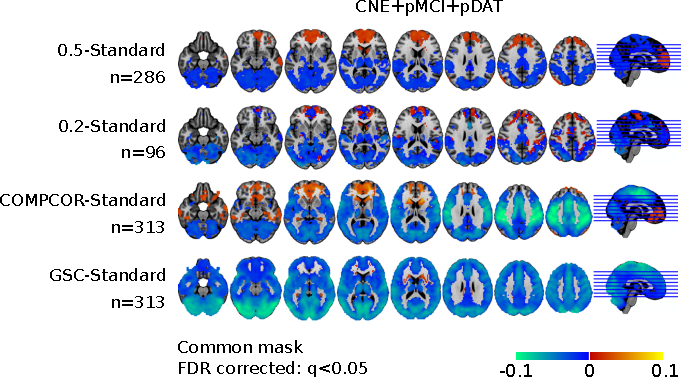
\includegraphics[width=\linewidth]{../figures/figure_comp.pdf}
\end{center}
\caption[Impact of the preprocessing on the DMN (CNE,pMCI,pDAT)]{
Differences in functional connectivity for the default mode network (seed in the PCC). Differences in connectivity between all the groups pooled together (CNE, pMCI, pDAT) with scrubbing ($FD>0.5$ and $FD>0.2$), CompCor, and GSC. The mask used depicts only significant result of the $t$-test (FDR correction $q<0.05$) only the two scrubbing procedures use the union of their respective mask (common mask).
}
\label{fig_scrubbimpact}
\end{figure}

\begin{figure}[H]
\begin{center}
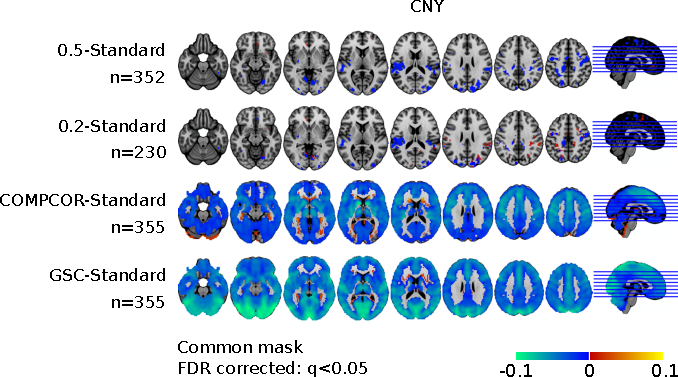
\includegraphics[width=\linewidth]{../figures/figure_comp_cny.pdf}
\end{center}
\caption[Impact of the preprocessing on the DMN (CNY)]{
{Differences in functional connectivity for the default mode network (seed in the PCC). Differences in connectivity between all the CNY with scrubbing ($FD>0.5$ and $FD>0.2$), CompCor, and GSC. The mask used depict only significant result of the $t$-test (FDR correction $q<0.05$) only the two scrubbing procedures use the union of there respective mask (common mask).}
}
\label{fig_sup_scrubbimpact_cny}
\end{figure}

\paragraph{Population specific impact of scrubbing}
The population specific difference in connectivity (see Figure \ref{fig_sup_impact_on_groups}) show almost identical findings as the combination of CNE, pMCI and pDAT therefore confirming that the observation are transferable in every population and not specific. Although the increase connectivity of the MPFC is observed in all groups when scrubbing is applied, the difference in connectivity is greater as we progress toward dementia (difference in fc for MPFC area CNE < pMCI < pDAT ). Difference map for CompCor and GSC revealed an invers patern where the greatest changes are observed in the CNE group followed by pMCI and finally pDAT for negative differences. CompCor show a increase in connectivity for the ACC area in the three groups but particularly in the pMCI group followed by CNE and then pDAT.


\begin{figure}[H]
\begin{center}
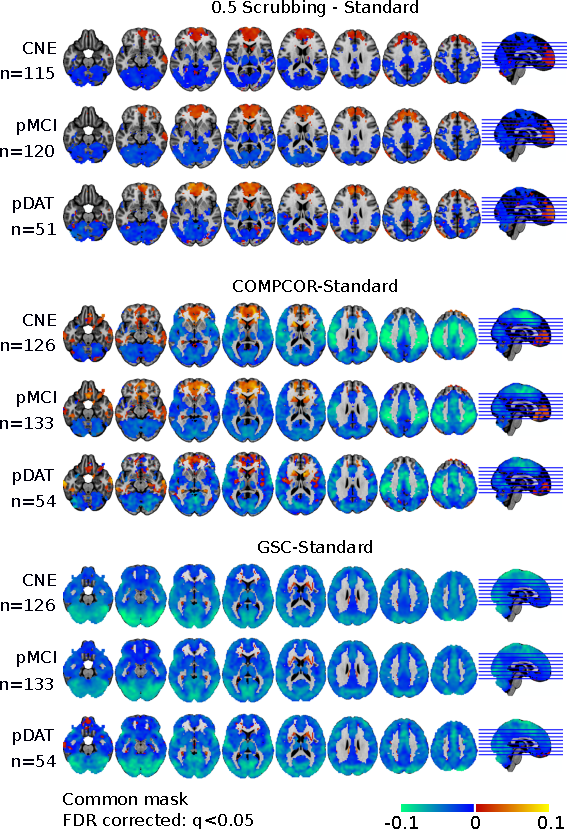
\includegraphics[width=0.75\linewidth]{../figures/scrubbing_impact_cne_mci_dat_all.pdf}
\end{center}
\caption[Impact of preprocessing on each group]{
{Differences in functional connectivity for the default mode network (seed in the PCC). Differences in connectivity for each group (CNE, pMCI, pDAT) compared to baseline (standard preprocessing) with and without scrubbing ($FD>0.5$), CompCor, and GSC (FDR correction $q<0.05$) for all voxels showing a significant effect in at least one of the contrast.}
}
\label{fig_sup_impact_on_groups}
\end{figure}

In order to assess if the significant differences in connectivity between groups are affected by the preprocessing strategy we did a $t$-test on each preprocessing strategy for every contrast (pDAT-CNE \ref{fig_impact_pDAT-CNE}, pDAT-pMCI \ref{fig_impact_pDAT-pMCI} and pMCI-CNE \ref{fig_impact_pDAT-pMCI}).

\begin{figure}[H]
\begin{center}
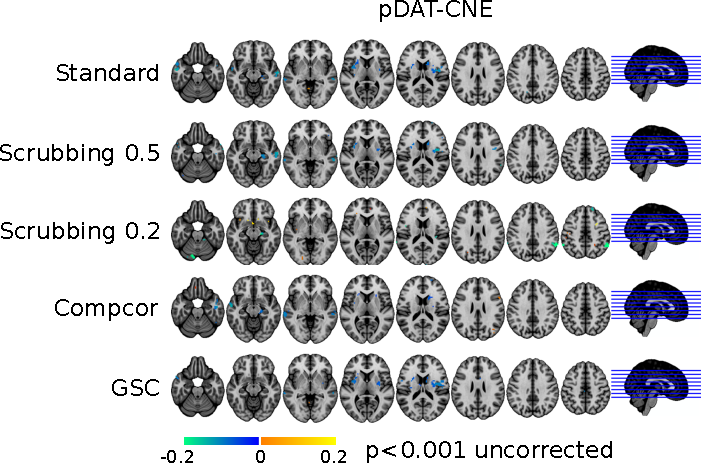
\includegraphics[width=0.60\linewidth]{../figures/scrubbing_impact_pDAT-CNE.pdf}
\end{center}
\caption[Scrubbing impact on group differences]{ Impact of preprocessing on connectivity differences between the pDAT and CNE groups. Connectivity differences between DMN ($t$-test p<0.001 uncorrected) computed with various preprocessing strategies (standard, scrubbing (0.5 and 0.2), CompCor and GSC).The maps are represented on top of the ICBM 152 anatomical atlas.
}
\label{fig_impact_pDAT-CNE}
\end{figure}

\begin{figure}[H]
\begin{center}
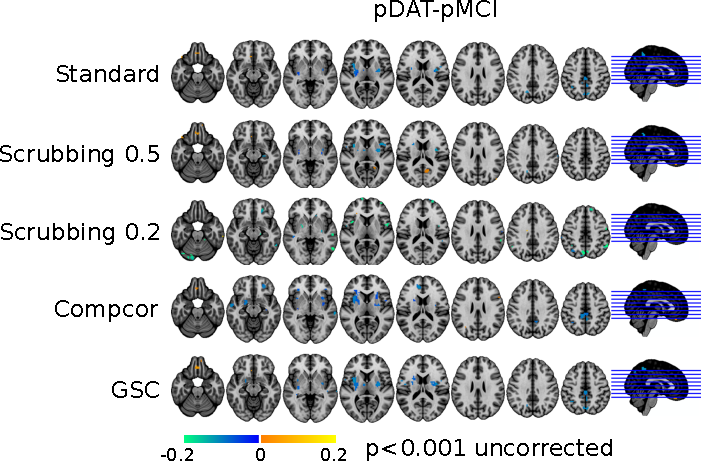
\includegraphics[width=0.60\linewidth]{../figures/scrubbing_impact_pDAT-pMCI.pdf}
\end{center}
\caption[Scrubbing impact on group differences]{ Impact of preprocessing on connectivity differences between the pDAT and pMCI groups. Connectivity differences between DMN ($t$-test p<0.001 uncorrected) computed with various preprocessing strategies (standard, scrubbing (0.5 and 0.2), CompCor and GSC).The maps are represented on top of the ICBM 152 anatomical atlas.
}
\label{fig_impact_pDAT-pMCI}
\end{figure}

\begin{figure}[H]
\begin{center}
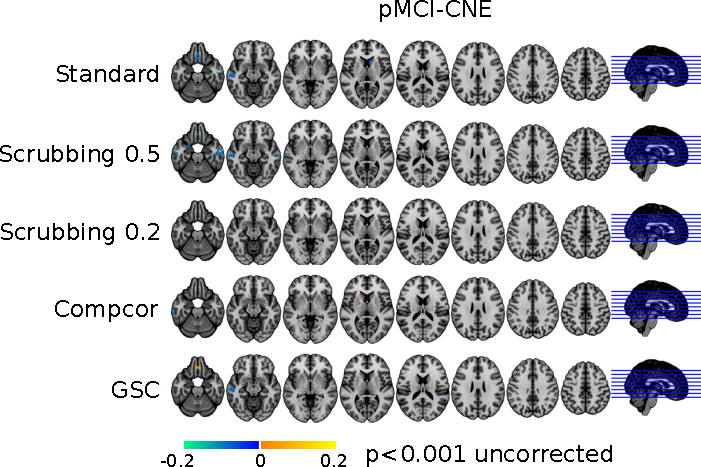
\includegraphics[width=0.60\linewidth]{../figures/scrubbing_impact_pMCI-CNE.pdf}
\end{center}
\caption[Scrubbing impact on group differences]{ Impact of preprocessing on connectivity differences between the pMCI and CNE groups. Connectivity differences between DMN ($t$-test p<0.001 uncorrected) computed with various preprocessing strategies (standard, scrubbing (0.5 and 0.2), CompCor and GSC).The maps are represented on top of the ICBM 152 anatomical atlas.
}
\label{fig_impact_pMCI-CNE}
\end{figure}


\subsection{Impact of scrubbing on our discriminative power between populations}
\paragraph{point to point connections}
Despite a moderate loss of subjects using a scrubbing at 0.5 (due to insufficient remaining data < 50 frames), the gains in data quality translated into an increased detection rate for group differences in almost all tested connections. As shown in Figure \ref{fig_p2p} the $FD\geq0.5$ scrubbing procedure mitigated motion artefacts and improved or maintain the statistical power of cross-sectional comparison of elderly clinical cohort. For $FD\geq0.2$ some improvement can be observed but the sample size remain too small to to be significant in most cases. The contrast with the most improvement due to scrubbing is the pDAT-CNE which is the contrast on which the literature point to point connections was selected for. For the pDAT-CNE contrast the most improved and consistent connections are connections with the IPL and the right SFG as well as the IPL and the dMPFC3. Connection with the PCC are also markedly improved by scrubbing namely the PCC and PCUN with MTL one of the first connection reported to be 
affected in the earliest stages of Alzheimer disease. Note that not all connection who had a good consistency with standard preprocessing improved using scrubbing. The statistical power for the pMCI-CNE contrast showed small improvements in PCC-PCUN, aMPFC-PCUN, IPL-dMPFC3 for $FD\geq0.5$ and improved consistency for SFGr-FUS with a scrubbing at $FD\geq0.2$. Finally the pDAT-pMCI contrast showed a general decrease in statistical power when scrubbing was applied, the only exception being aMPFC-PCUN that show improvement when a scrubbing at $FD\geq0.2$ was applied.

\paragraph{Detection power for every scrubbing strategy}
The simulation applied using CompCor and GSC preprocessing strategies revealed less consistency with the previously mentioned pairs of connections, especially for the pDAT-CNE contrast, that was supposed to be the optimized contrast with that selection of connection pairs. For the pMCI-CNE contrast, GSC was consistently outperformed by CompCor and Standard preprocessing in the most dominant connection, namely dMPFC-dMPFC2, PCC-PCUNm and aMPFC-MTL. On the other hand, in the last contrast pDAT-pMCI, the CompCor preprocessing was the preprocessing strategy with the most improved statistical power for aMPFC-PCUN, PCC-MTL and IPL-MTL. Interestingly, the scrubbing procedure seemed to improve the detection power more consistently and over a larger number of pair of connections than the CompCor and GSC methods (see Figure \ref{fig_p2p} and \ref{fig_sup_p2p_gsc_compcor}).


\begin{figure}[H]
\begin{center}
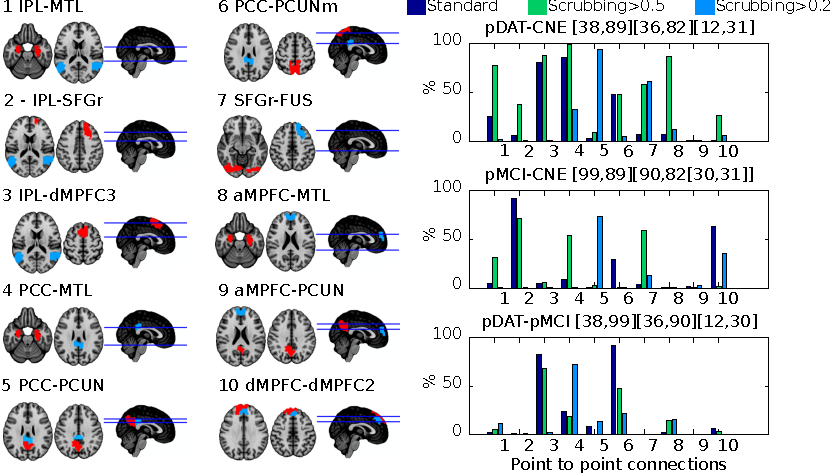
\includegraphics[width=\linewidth]{../figures/p2pdetection.pdf}
\end{center}
\caption[Detection power with Scrubbing]{
On the Left: Seeds from 10 point-to-point connections. PCC (posterior cingulate cortex), PCUN (precuneus), dMPFC (dorsomedial prefrontal cortex), dMPFC2 (dorsomedial prefrontal cortex2), IPL (inferior parietal lobule), SFGr (right superior frontal gyrus), aMPFC (anterior medial prefrontal cortex), PCUNm (precuneus motor), dMPFC3 (dorsmedial prefrontal cortex3), MTL (Mesial temporal lobe). On the right: Detection power of group differences for 3 preprocessing strategy (standard, scrubbing $FD>0.5$ and scrubbing $FD >0.2$). The detection power is computed using a $t$-test of each connection ($p<0.05$) replicated $B=10^4$ times using random subsamples of 70\% of each group. Explanatory variables included age and gender and a multi-site bias correction are applied.
}
\label{fig_p2p}
\end{figure}

\begin{figure}[H]
\begin{center}
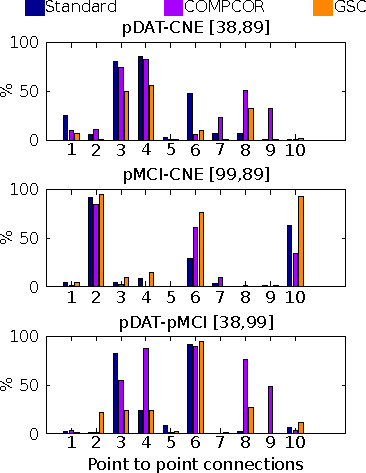
\includegraphics[width=0.5\linewidth]{../figures/p2pdetection_gsc_compcor.pdf}
\end{center}
\caption[Detection power with CompCor and GSC]{
Detection power of group differences for 3 preprocessing stategy (standard, CompCor and GSC). The detection power is computed using a $t$-test of each connection ($p<0.05$) replicated 10,000 times using random subsamples of 70\% of each group. Explanatory variables included age and gender and a multi-site bias correction are applied.
}
\label{fig_sup_p2p_gsc_compcor}
\end{figure}


\section{Conclusion} We observed that motion introduced a systematic bias in the measures of resting-state connectivity in elderly population. Populations suffering did not exhibit more severe motion level than cognitively normal elderly subjects. The scrubbing procedure mitigated motion artefacts and improved the statistical power of the detection of differences in average functional connectivity between clinical populations.


\chapter{Feasibility of multi-centric fMRI connectivity studies of Alzheimer's disease}

My second on-going project investigates the multi-site bias in connectivity measures, and the methods that can be used to reduce this bias. Part of this work was publised in the proceedings of the Alzheimer's Association International Conference (AAIC) \cite{Dansereau2013}, and a full-length manuscript is currently in preparation. 

\section{Introduction}
Resting-state (RS) connectivity in fMRI is a promising biomarker for a variety of neurological diseases. Typically, in a clinical trial, a large cohort is recruited and evaluated at multiple sites spread over countries or even continents. The main potential issue with that approach is the lack of consistency in the multi-site RS connectivity acquisitions that may obscure clinically relevant information. Therefore the aims of the study were to: (1) characterize the amplitude of the site bias, i.e. the systematic differences in rs-fMRI connectivity across different acquisition sites; (2) Quantify the impact of the between-site variance on the power of statistical tests in resting-state fMRI.

\section{Method}

\subsection{Preprocessing}\label{Preprocessing}
The datasets were analysed using the NeuroImaging Analysis Kit (NIAK\footnote{\url{http://www.nitrc.org/projects/niak/}}) version 0.12.14, under CentOS version 6.3 with Octave\footnote{\url{http://gnu.octave.org}} version 3.8.1 and the Minc toolkit\footnote{\url{http://www.bic.mni.mcgill.ca/ServicesSoftware/ServicesSoftwareMincToolKit}} version 0.3.18. Analyses were executed in parallel on the "Mammouth" supercomputer\footnote{\url{http://www.calculquebec.ca/index.php/en/resources/compute-servers/mammouth-parallele-ii}}, using the pipeline system for Octave and Matlab \citep{Bellec2010}, version 1.0.2. Brain map visualizations were created using MRICron software \cite{Rorden2007}. Each fMRI dataset was corrected of inter-slice difference in acquisition time and the parameters of a rigid-body motion was estimated for each time frame. Rigid-body motion was estimated within as well as between runs, using the median volume of the first run as a target. The median volume of one selected fMRI run for each subject 
was 
coregistered with a T1 individual scan using Minctracc \citep{Collins1998}, which was itself non-linearly transformed to the Montreal Neurological Institute (MNI) template \citep{Fonov2011} using the CIVET pipeline \citep{Zijdenbos2002}. The MNI symmetric template was generated from the ICBM152 sample of 152 young adults, after 40 iterations of non-linear coregistration. The rigid-body transform, fMRI-to-T1 transform and T1-to-stereotaxic transform were all combined, and the functional volumes were resampled in the MNI space at a 3 mm isotropic resolution. The a censoring method described in \citep{Power2012} called "scrubbing" was used to remove the volumes with excessive motion using a cut-off value of $FD\geq0.5$. A minimum number of 50 unscrubbed volumes per run, corresponding to $\sim 125$ s of acquisition for a TR of 2.5 seconds, was then required for further analysis. The following nuisance parameters were regressed out from the time series at each voxel: slow time drifts (basis of discrete cosines 
with a 0.01 Hz high-pass cut-off), average signals in conservative masks of the white matter and the lateral ventricles as well as the first principal components (95\% energy) of the six rigid-body motion parameters and their squares \citep{Lund2006},\citep{Giove2009}. The fMRI volumes were finally spatially smoothed with a 6 mm isotropic Gaussian blurring kernel. 

\subsection{Feature selection}
Regions are routinely defined using an anatomical parcellation \citep{He2009}, such as the AAL template \citep{Tzourio-Mazoyer2002}. Anatomical parcels may however not well match the organization of resting-state networks. The BASC method was used to generate data-driven functional decomposition into resting-state networks based on the coherence of BOLD activity at the individual or group level \citep{Bellec2006,Bellec2010c,Bellec2013}. When a low number of networks (or scale) is used, the brain got decomposed into distributed large-scale networks, such as the DMN. At high scales (large number of networks), the BASC identified subnetworks and functional regions \citep{Kelly2012}. We generated a BASC parcellation in 100 clusters on the Cambridge sample, including $\sim 200$ young adults from the 1000 functional connectome database \citep{Biswal2010} and used it to generate the rs-fMRI outcome measures.

\paragraph{The default-mode network}
Since the seminal work of \cite{Greicius2004}, many rs-fMRI studies in AD focused on the default-mode network (DMN), a group of regions consistently more active at rest than during a broad range of different tasks \citep{Gusnard2001}. The DMN was notably reported to largely overlap with the regions that show high amyloid-beta deposition in patients with DAT \citep{Buckner2009}. It includes the posterior cingulate cortex (PCC) / Precuneus (PCUN) area, the inferior parietal lobule (IPL), the anterior cingulate cortex / medial prefrontal cortex (MPFC) \citep{Greicius2003}. Other structures such as the medial temporal cortex or the superior frontal gyrus are also generally regarded as part of different subnetworks of the DMN \citep{Margulies2009, Andrews-Hanna2010a}.

\paragraph{Literature review: Alzheimer's disease and resting-state fMRI}
We performed a literature review to select candidate connections that have been shown to be prominently impacted in Alzheimer's disease. There is no single authoritative reference on the effect of a DAT on rs-fMRI connectivity, and the field has been dominated thus far by studies with small samples (n\textasciitilde20) and limited statistical power, see \cite{Sheline2013} for a recent review. Because the DMN has been most extensively studied, we decided to focus on this network and to run a meta-analysis on six papers that (1) used some analogue of seed-based connectivity maps in resting-state fMRI using one or multiple seeds in the DMN (2) investigated abnormalities in resting-state functional connectivity in patients suffering of a dementia of the Alzheimer's type and (3) provided tables of coordinates in stereotaxic space for the results.

\paragraph{review: Alzheimer's disease and resting-state fMRI} 
\begin{itemize}
\item \cite{Zhang2009a} used functional connectivity maps with a seed in the posterior cingulate cortex (PCC) to explore the differences between a group of elderly cognitively normal subjects (CNE, n=16) and patients with a mild dementia of the Alzheimer's type (DAT, n=18).
\item \cite{Zhang2010} generalized the \cite{Zhang2009a} study with CNE (n=16) and a larger group of patients with DAT (n=46). Patients were separated in three groups (mild, moderate, severe DAT), and each group of patients was contrasted against the CNE.
\item \cite{Wang2006a} used functional connectivity maps with a seed in the hippocampi to explore the differences between a group of CNE (n=13) and patients with a mild DAT (n=13). All results included in the meta-analysis are from Table 2, seeded in the right hippocampus. Seeds were manually delineated on an individual basis.
\item \cite{Wang2007a} used functional connectivity maps with a seed in the posterior cingulate cortex (PCC) as well as full brain point-to-point correlations (based on an AAL parcellation) to explore the differences between a group of elderly cognitively normal subjects (CNE, n=14) and patients with a very mild to mild dementia of the Alzheimer's type (DAT, n=14). Only the results based on the PCC seed were included in the meta-analysis.
\item \cite{Goveas2011} used functional connectivity maps with a seed in the hippocampi to explore the differences between a group of elderly cognitively normal subjects (CNE, n=18) and patients with a mild dementia of the Alzheimer's type (DAT, n=14) before and after donepezil treatment. Seeds were manually delineated on an individual basis, before and after treatment.
\item \cite{Damoiseaux2012} used dual-regression independent component analysis to explore longitudinal differences between a group of CNE (n=18) and patients with DAT (n=21). All results included in the meta-analysis are from Table 3 (differences at baseline) and Table 4 (interaction with time). The authors used three components representing the Anterior DMN, Ventral DMN and Posterior DMN.
\end{itemize}

To assess the degree of consistency of the findings across studies, we counted the number of coordinates located in each one of the BASC regions. The resulting map is presented in Figure \ref{fig_freq_sel}. As can be seen, there is a lot of variability across studies, with only a limited number of regions reaching a score above 3 (i.e. reported in at least 3 of the contrasts in the six studies). Note that we did not select connections with the hippocampus, although this region was frequently reported. The rationale was that the drug effects on this area are expected to be minimal in patients with a moderate DAT, because the very severe atrophy of the structure cannot be recovered. In the regions showing the most consistency (score of 3 or more), there were many regions located in the DMN, such as the PCC, the PCUN, the IPL (a bilateral node), the right superior frontal gyrus (SFGr), as well as two dorsal MPFC cortex (dMPFC and dMPFC2) and an anterior MPFC parcel (aMPFC). Three parcels were found in the 
visual network: the lingual gyrus (LING), the fusiform gyrus (FUS) and a dorso-medial occipital (DMO) parcel. Two parcels were found in the dorsal attentional network: the intra-parietal sulcus (IPS) and the motor part of the precuneus (PCUNm, see \cite{Margulies2009}). One parcel was found in the premotor cortex (PMC), associated with the sensorimotor network, one parcel in the left dorsolateral prefrontal cortex (rDLPFC), associated with the fronto-parietal task-control network, as well as a parcel in the dMPFC (dMPFC3) associated with the cingulo-opercular cortex. Finally, a parcel included the temporal poles (TPo) bilaterally. Note that the nomenclature for distributed networks was based on \citep{Power2011}. 

The TRT reliability study was based on the publicly available NYU-TRT database. The database included 25 young healthy adults, and each subject had three rs-fMRI run: two in a single session (separated by 45 mns) and another run $5-16$ months latter. Several outcome measures were generated in key regions impacted by AD. Using the three runs, one intra-class correlation (ICC) was generated intra-session, and two ICCs were generated inter-session for each outcome measures. The outcome measures were ranked based on average of intra- and inter-session ICCs. 

\subsection{Simulations}
\paragraph{Dataset}
In order to simulate various scenarios within the context of a multi-site setting, a cohort of subjects acquired at a single-site was selected to act as our reference dataset and for the multi-site configuration a cohort from a collection of 7 small sites, roughly totalling the same sample size as the reference dataset, was used. The cohort used for the study contains 385 participants from the 1000 Functional Connectomes Project \citep{Biswal2010} (150 males, age range = 18-46 yrs) composed of 1 large site (Cambridge n=\textasciitilde200) and 7 small sites (n=\textasciitilde20/site for a total \textasciitilde200). The fMRI datasets were preprocessed with the Neuro-Imaging Analysis Kit (NIAK) as described earlier in Section \ref{Preprocessing}.

\paragraph{Connectome}
Using a brain partition of $R$ networks obtain from BASC procedure described in \cite{Bellec2010c}, and taking each pair of distinct networks $i$ and $j$, the between-network connectivity $y_{i,j}$ is measured by the Fisher transform of the Pearson's correlation between the average time series of the network. The within-network connectivity $y_{i,i}$ is the Fisher transform of the average correlation between time series of every pair of distinct voxels inside network $i$. The connectome $\mathbf{Y}=(y_{i,j})_{i,j=1}^R$ is thus a $R\times R$ matrix. Each column $j$ (or row, as the matrix is symmetric) codes for the connectivity between network $j$ and all other brain networks (full brain functional connectivity map). For a scale with $R$ parcels, there are exactly $L=R(R+1)/2$ distinct elements in an individual connectome $\mathbf{Y}$. 

\paragraph{Effect size (cohen's d)}
For each site and each sample, half of the subjects were randomly assigned to a "treatment" group and a Monte-Carlo simulation was used to estimate the detection power in the single-site and in multi-site setting.

The normalized Cohen's d was used to estimate the effect size and it is defined as the difference between two means $\bar{x_{1}},\bar{x_{2}}$ divided by a standard deviation from the data $s$.

\begin{equation}\label{cohen's d}
    \begin{array}{l l}
      s = \sqrt{\frac{(n_{1}-1)s_{1}^{2}+(n_{2}-1)s_{2}^{2}}{n_{1}+n_{2}-2}} \\
      d = \frac{\bar{x_{1}}-\bar{x_{2}}}{s}
    \end{array}
\end{equation}

$n_{1}$ and $n_{2}$ are the respective number of subject in each group. In order to introduce the same effect-size across the single-site and multi-site dataset we are taking the standard deviation from the single-site cohort as the reference.  The connection $y_{i,j}$ of the randomly affected subjects ("treatment" group) are therefore calculated $y_{i,j} = y_{i,j} + d\times s_{i,j}$. The significance of the difference between the control and 'treatment' group was assessed by a $t$-test in a linear model, including a covariate to model the motion. The study was repeated for various effect sizes (0 to 0.8 with a step of 0.01) with a $p$-value threshold of $0.05$ on the $t$-test.

\paragraph{multi-site correction approaches} 

For the multi-site three flavours were computed: multi-site no correction, multi-site with dummy variables and multi-site with METAL correction.
Depending on the multi-site configuration and distribution of the subject we proposed two corrective approaches that can be applied as shown in the simulations of Figure \ref{fig_simu_50pct}. The first one is the introduction of dummy variables (binary vectors $1\times N$) who code for each site in the GLM model \ref{dummy variable equation}.

The variables are corrected to have a zero mean across subjects, and an intercept (i.e. a column filled with 1) is added to $\mathbf{X}$. The GLM relies on the following stochastic model:
 \begin{equation}
 \label{eq_glm}
  \mathbf{Y} = \mathbf{X}\mathbf{\beta} + \mathbf{E}
 \end{equation}
where $\mathbf{\beta}$ is an unknown $C\times L$ matrix of linear regression coefficients and $\mathbf{E}$ is a $N\times L$ random (noise) multivariate Gaussian variable. %As data generated from different subjects are statistically independent, and under an homoscedasticity assumption, the regression coefficients $\mathbf{B}$ can be estimated with ordinary least squares.
To apply the correction $v-1$ dummy-variables are added to the model \ref{dummy variable equation} with $v$ being the total number of sites used in the study.

\begin{equation}
    y_{i,j} = \beta x+\beta_{i=1,\dots,v-1}x_{i=1,\dots,v-1}+e
    \label{dummy variable equation}
\end{equation}

The second approach is to compute the GLM independently on each site and then combine the statistical results from each site in a global score. This model averaging technique called METAL from \cite{Willer2010} model site specific bias by running a GLM analysis on each site resulting in $v$ beta vectors that are weighted proportionally to the standard error of each site and finally averaged as shown in equation \ref{METAL}. This is the most flexible way to account for multi-site effect wile keeping the analysis simple and robust to unbalanced sites.


\begin{equation}
	\beta_{v} \text{, effect size estimate for site \textit{v}.}
\end{equation}
\begin{equation}
	se_{v} \text{, standard error for site}\textit{v}.
\end{equation}
\begin{equation}
 	w_{v}=\frac{1}{se_{v}^{2}} \text{, weight estimate for site \textit{v}.}
 \end{equation}
 \begin{equation}
 	SE=\sqrt{\frac{1}{\Sigma_{v}w_{v}}} \text{, global standard error.}
 \end{equation}
 \begin{equation}
 	\beta=\frac{\Sigma_{v}\beta_{v}w_{v}}{\Sigma_{v}w_{v}} \text{, global }\beta.
 \end{equation}
\begin{equation}\label{METAL}
	Z=\frac{\beta}{SE} \text{, global Z score.}
\end{equation}
\begin{equation}
	p=2(1-\phi(\vert Z \vert) \text{, p-value.}
\end{equation}

\section{Results}

The Figure \ref{fig_icc} presents the results of the ICC analysis for the point-to-point correlations, 
%(a), regional clustering (b), regional degree centrality (c), global summary such as the average clustering, average efficiency and modularity (d) and local efficiency (e). 
only the connections with an average ICC above 0.5 are represented. The results were consistent with \citep{Shehzad2009}, with a mean ICC over all connections of \textasciitilde0.3 and 23 connections scoring a moderate-to-good level of ICC ($>0.5$). 

\begin{figure}[H]
\begin{center}
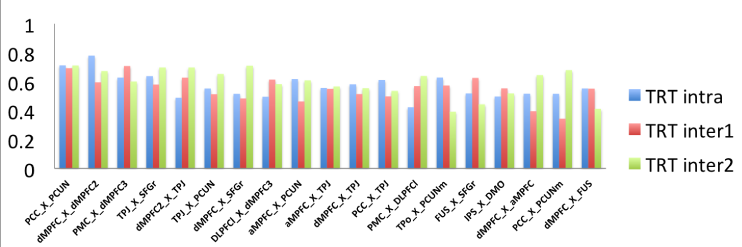
\includegraphics[width=\linewidth]{../figures/fig_icc.png}
\end{center}
\caption[ICC scores]{
  ICC scores for pairs of connections passing the $>0.5$ threshold on the NYU-TRT dataset.
}
\label{fig_icc}
\end{figure}

Average connectivity maps associated with the DMN nodes as well as the nodes outside the DMN that passed the TRT selection are presented in Figures \ref{fig_nodes_DMN} and \ref{fig_nodes_none_DMN}. The involvement of the sensorimotor, visual and attentional networks mainly came from contrasts reporting a decrease of negative correlations in patients, that was interpreted as a compensation mechanism by some authors. These connections are potentially very valuable to monitor the effect of a drug. Considering that we pooled studies of the DMN, we decided to select as candidates all connections of parcels within the DMN, as well as connections between a parcel inside the DMN and a parcel outside the DMN. The final selection of target measures was based on test-retest reliability. All the parcels and associated labels and networks are listed in Table \ref{tab_point-to-point}.


\begin{figure}[H]
\begin{center}
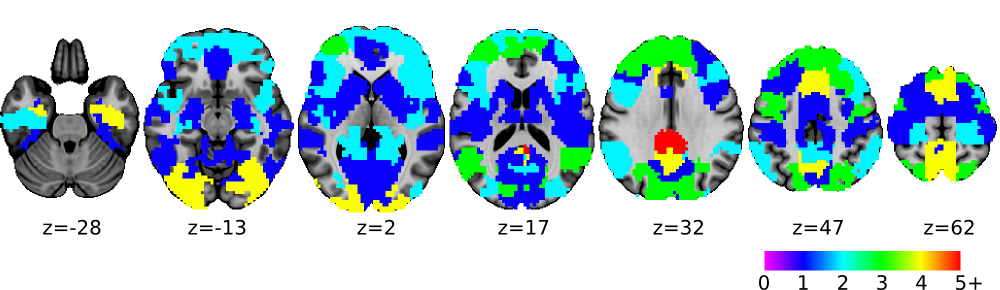
\includegraphics[width=\linewidth]{../figures/fig_freq_sel_dat.png}
\end{center}
\caption[Cited region frequency]{
  Frequency of reported regions showing functional differences based on a literature review of 6 papers.
}
\label{fig_freq_sel}
\end{figure}

\begin{figure}[H]
\begin{center}
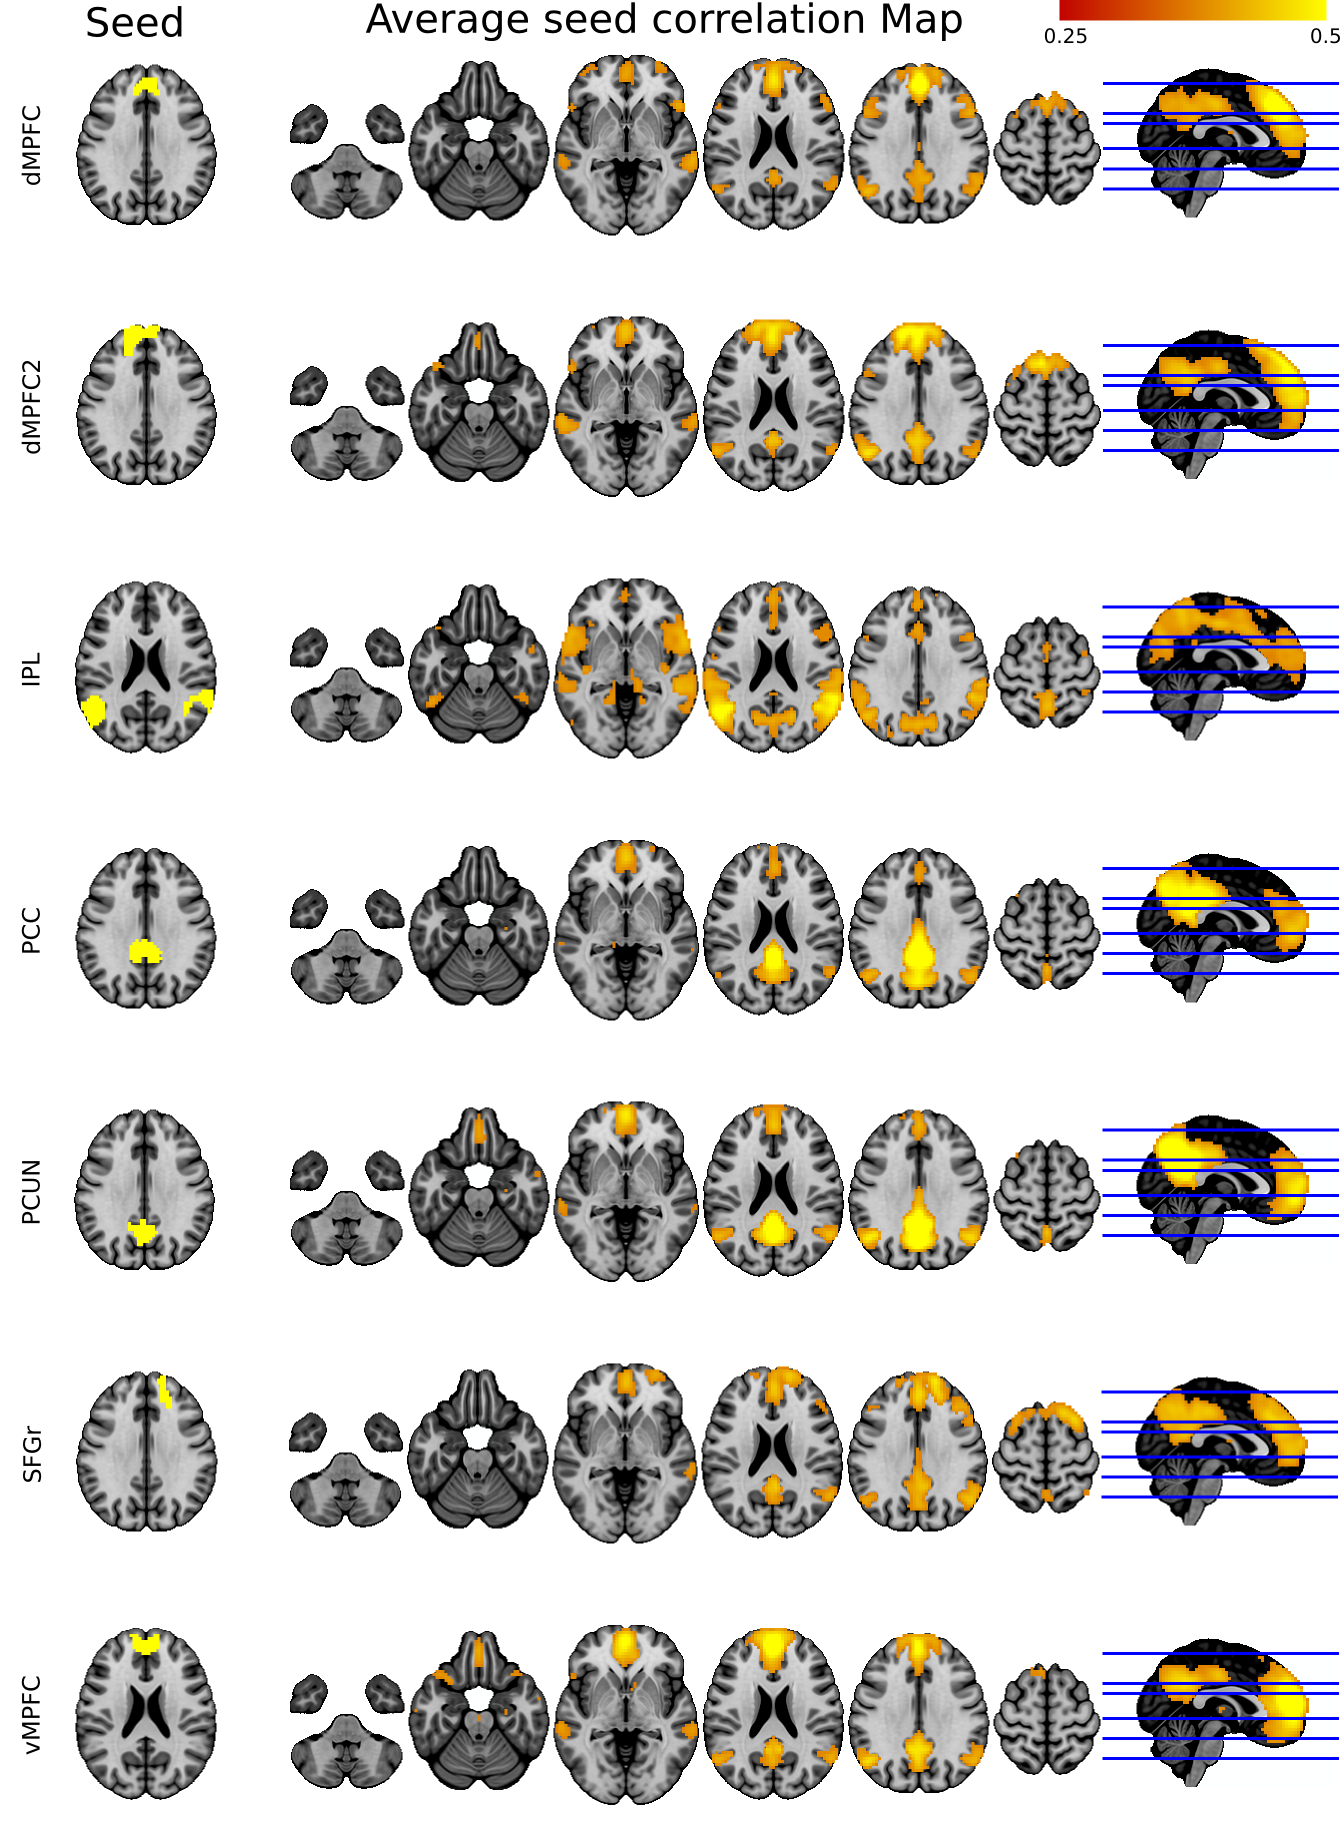
\includegraphics[width=\linewidth]{../figures/fig_nodes_DMN.png}
\end{center}
\caption[Selected region inside DMN]{
  Selected nodes inside the DMN who passed the TRT selection.
}
\label{fig_nodes_DMN}
\end{figure}

\begin{figure}[H]
\begin{center}
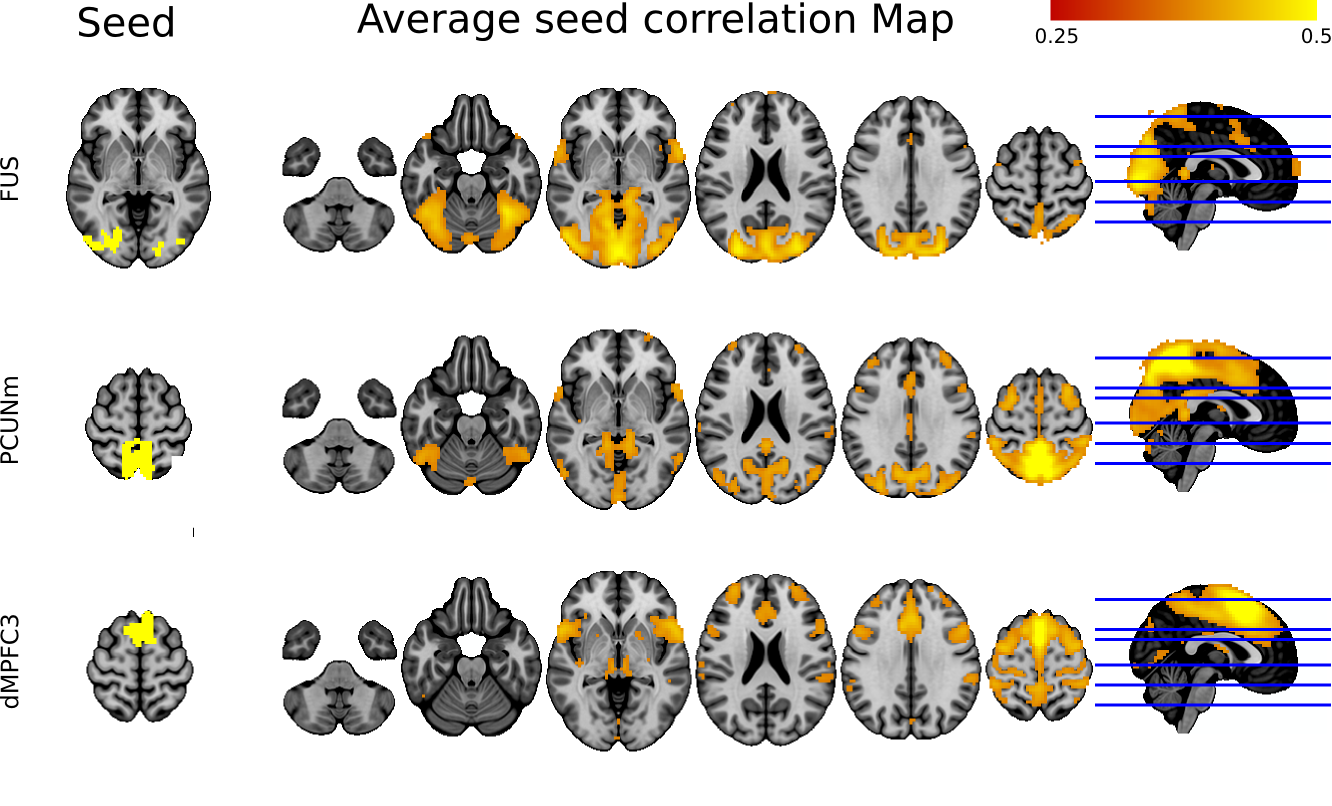
\includegraphics[width=\linewidth]{../figures/fig_nodes_non_DMN.png}
\end{center}
\caption[Selected region outside DMN]{
	  Selected nodes outside the DMN who passed the TRT selection.
}
\label{fig_nodes_none_DMN}
\end{figure}
%Regarding the graph measures, there is a growing arsenal of metrics that have been proposed in the literature, see \citep{Bullmore2009} for a review, notably box 2 for a summary of measures. We selected some of the most standard metrics that have been shown (or suggested) to be impacted by a disease of the Alzheimer type. Regarding local measures, \cite{Buckner2009} noted the similarity of the “degree centrality”, or “hubs” maps in young adults and the patterns of deposition of amyloid-beta in patients suffering of a DAT. This work (or subsequent work as far as we know) did not test directly the relationship between degree centrality and the presence/progress of DAT. An important paper for our purposes is \cite{Supekar2008}, that showed that both local and global clustering coefficients (but not efficiency) are impacted by a DAT. By contrast, \cite{Sanz-Arigita2010} reported that global efficiency (and not global clustering) was impacted by DAT. This inconsistency may simply reflect the low 
%statistical power shared by both studies (18 ECN, 21 patients with mild DAT for the former paper, and 21 ECN, 18 patients with mild DAT for the latter), or methodological differences. Finally, we also included the measure of modularity \citep{Rubinov2011}, a promising tool that has not been used yet in DAT. We used the implementation of the metrics described in \cite{Rubinov2011}. Note that all the metrics first require to binarize the functional connectome of each participant, which was achieved with a density-based threshold (top 20\% positive connections, see the test-retest section below for a rationale).

%In total, the literature review identified 7 nodes in the DMN (21 point-to-point correlations within the DMN) and 9 seeds in networks outside of the DMN (63 point-to-point correlations between a node in the DMN and a node outside of the DMN). We included three local network properties in the DMN (21 measures), as well as two global properties. That's a total of 107 candidate measures, based on a fairly conservative literature review. We further analyzed the test-retest reliability of these measures to narrow the selection down to about 10 measures. 

%The literature on TRT reliability of graph measures is much more difficult to interpret: \cite{Braun2012} for example has included many possible strategies to generate graph properties, resulting into almost the full range of possible ICC values for every metric ! Because no processing strategy was an obvious winner across all metrics, we selected the middle thresholding (20\% density) of \cite{Braun2012}. The relatively low ICC for graph measures (only a few measures with $ICC>0.5$, many measures with $ICC < 0.2$), was consistent with the results of \citep{Wang2011}.

\begin{table}[H]
\begin{center}
\begin{tabular}{l l l l}
\bfseries{Network} & \bfseries{Label} & \bfseries{Name} & \bfseries{Cambridge100}\\
\hline
 & PCC & posterior cingulate cortex & 1\\
 & dMPFC & dorsomedial prefrontal cortex & 12\\
 & dMPFC2 & dorsomedial prefrontal cortex & 46\\
Default-mode network & aMPFC & anterior medial prefrontal cortex & 42\\
 & IPL & inferior parietal lobule & 49\\
 & PCUN & precuneus & 53\\
 & MTL & medial temporal lobe & 39\\
 & SFGr & right superior frontal gyrus & 76\\
\hline
Visual network & FUS & fusiformgyrus & 71\\
\hline
Dorsal attentional & PCUMm & precuneus (motor) & 94\\
\hline
Cingulo-opercular network & dMPFC3 & dorsmedial prefrontal cortex & 90\\
\end{tabular}
\end{center}
\caption{Regions selected in the literature review, the region number correspond to the number in the Cambridge 100 partition.}
\label{tab_point-to-point}
\end{table}

For point-to-point correlations within the DMN, we selected the connections with highest ICC for each node (all average ICC > 0.5):
\begin{itemize}
\item PCC x PCUN
\item dMPFC x dMPFC2
\item IPL x SFGr
\item aMPFC x PCUN
\end{itemize}
For each point-to-point correlation between the DMN and another network, we selected the connections with highest ICC and ICC > 0.5:
\begin{itemize}
\item FUS x SFGr
\item PCC x PCUNm
\item IPL x dMPFC3
\end{itemize}
% The only graph properties that satisfied the above criteria were:
% \begin{itemize}
% \item[•] average clustering
% \item[•] clustering PCUN
% \item[•] local efficiency PCUN
% \end{itemize}


The first assessment perform on the dataset was to verify the distribution of the variance in functional connectivity among each site and across sites in order to see if they are of the same order of magnitude or not. This analysis of Figure \ref{fig_site_variability} shows the distribution of the standard deviation of connectivity across subjects (the distribution is over the full brain connectome, with several 1000s connections) at the 8 sites against the inter-sites standard deviation of connectomes (average at each site). as we can see the inter-site (between site) variability is smaller than the intra-site (between subjects) variability.

\begin{figure}[H]
\begin{center}
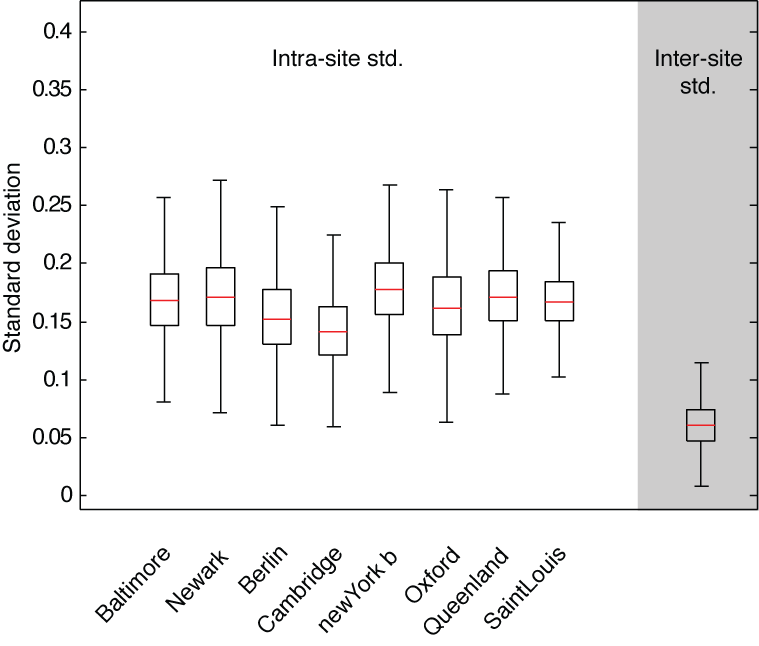
\includegraphics[width=\linewidth]{../figures/inter_vs_intra_3tonly.png}
\end{center}
\caption[inter vs. intra site variability]{
  Distribution of intra-site (between-subject) standard deviation vs. inter-site (between-site) standard deviation, based on the standard deviation of the connectivity matrices from 8 sites from the 1000 functional connectome dataset.
}
\label{fig_site_variability}
\end{figure}

In order to verify how spatial structure vary across sites the average standard deviation and the average connectivity map of the DMN was extracted for each site and displayed in Figure \ref{fig_DMN_variability}. In order to ease the reading we selected only 4 representative sites, although we reached the same conclusion on all the sites. As we can see in the intersection between two sites the difference in standard deviation between-sites was illustrated (red set of brain cuts). First the mean DMN at each site is consistent with the expected spatial ditribution reported in other studies. As we can see the amplitude of inter-site bias is about 3-fold smaller than the within-site standard deviation (red \textasciitilde0.06 vs. orange \textasciitilde0.18). The most salient changes between-sites are located in the mesio-frontal region associated with the anterior part of the DMN. This last finding may be associated with motion artefact as previously reported in \cite{Dansereau2014}.

\begin{figure}[H]
\begin{center}
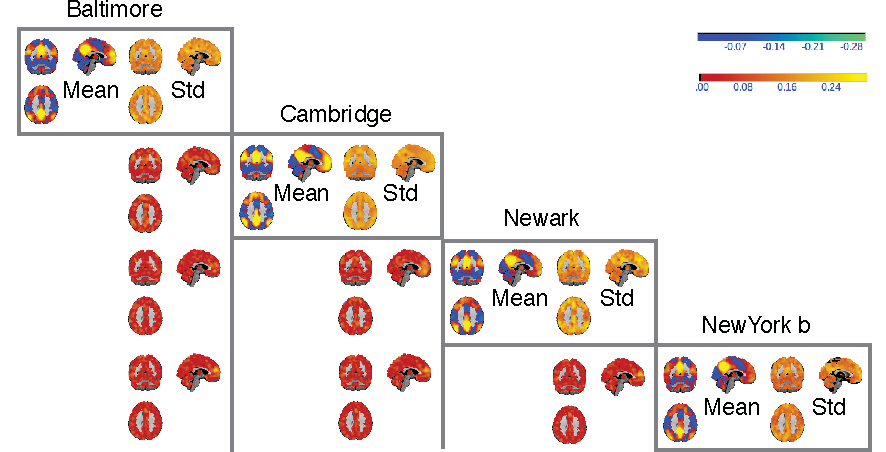
\includegraphics[width=\linewidth]{../figures/mult_center_dm_voxel_seed_3tonly.pdf}
\end{center}
\caption[DMN variability across sites]{
Functional connectivity maps of the default-mode network at multiple sites. The average connectivity map for 4 sites (Baltimore, Cambridge, Newark and New-Yorkb at 3T) are presented on the diagonal (left). The standard deviation across subjects and within site is presented next to it (diagonal squares, right part). Each off-diagonal block represent the absolute difference between the average functional connectivity maps between two sites (called the inter-site bias).
}
\label{fig_DMN_variability}
\end{figure}

We also showed using Monte-Carlo simulations that the power of detecting an effect is marginally affected by the site acquisition configuration (single site or multi-site, see Figure3.2 for an illustration of a power analysis on three different seeds) where the sites are balanced in term of the amount of subject with and without the effect. 

\begin{figure}[H]
\begin{center}
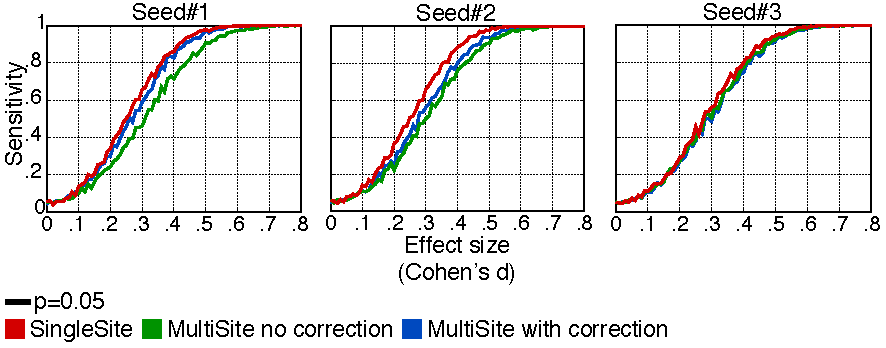
\includegraphics[width=\linewidth]{../figures/simu_results_multisite.pdf}
\end{center}
\caption[Detection power]{
Power analysis for a resting-state fMRI study. A Monte-Carlo simulation was implemented to evaluate the power of a resting-state multi-site study, based on real values of three connections in the default-mode network PCC/MFC, rHIP/vMFC and lIPC-rDLPFC. For each site and each sample, half of the subjects were randomly assigned to a 'treatment' group. For the subjects in this group, a value was added to achieve a given relative effect size (Cohen's d, i.e. the mean of the two groups divided by the standard deviation of all sites). The significance of the difference between the control and 'treatment' group was assessed by a $t$-test in a linear model, including covariates to model site-specific bias. The study was repeated for various effect sizes (0 to 0.8 with a step of 0.01) at a threshold of 0.05 on the p-value in the $t$-test. For a p of 0.05, a statistical power of 0.
95 can be achieved for as low as a 0.47 effect size. The simulation was based on a scenario with 8 sites and 385 subjects, and no homogeneization of acquisition protocol whatsoever. The multi-site (with and without correction) is based on 187 subjects from 7 sites and the SingleSite is based on one site of 198 subjects. 
}
\label{fig_detection_power}
\end{figure}

\begin{figure}[H]
\begin{center}
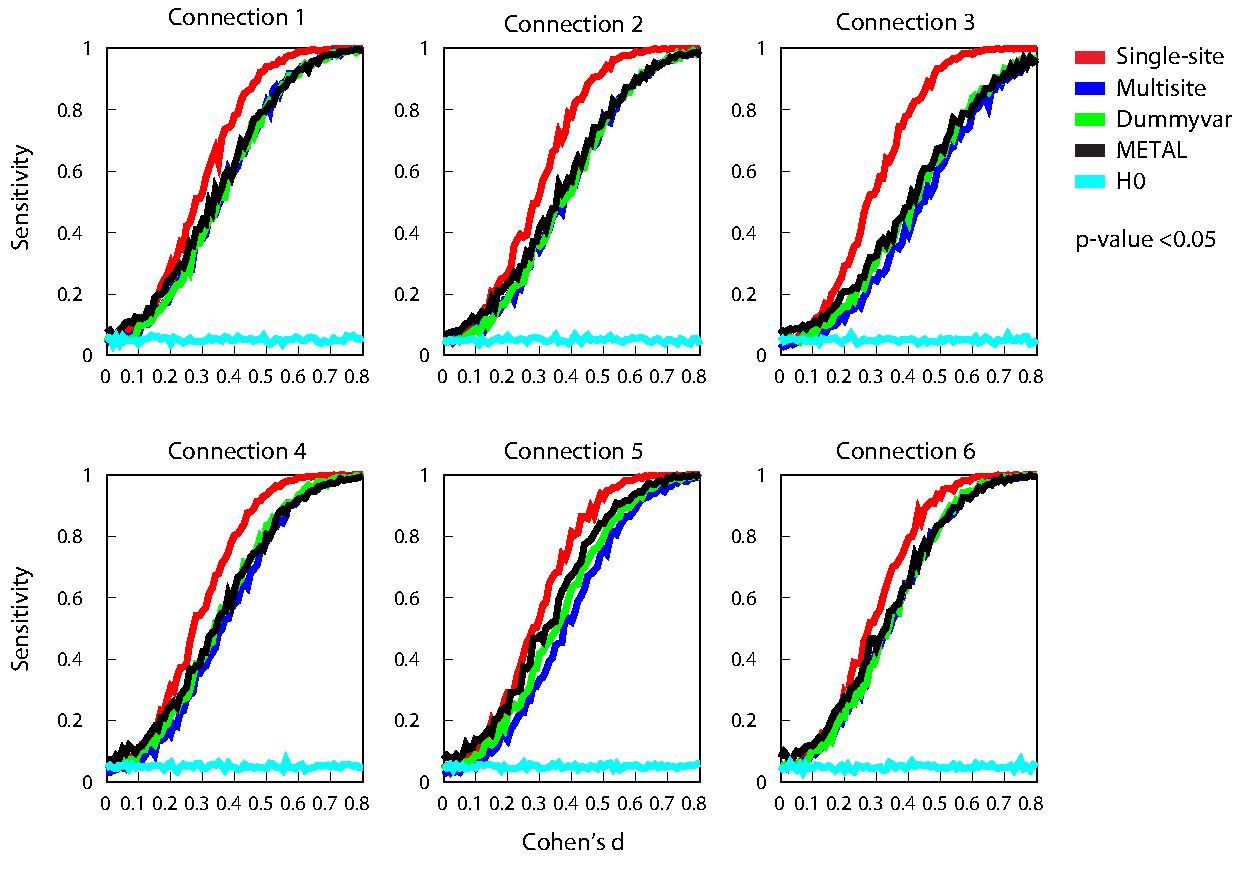
\includegraphics[width=\linewidth]{../figures/multisite_simulation_50pct.pdf}
\end{center}
\caption[Detection power 2]{
Power analysis for a resting-state fMRI study. A Monte-Carlo simulation was implemented to evaluate the power of a resting-state multi-site study. For each site and each sample, half of the subjects were randomly assigned to a 'treatment' group. For the subjects in this group, a value was added to achieve a given relative effect size (Cohen's d, i.e. the mean of the two groups divided by the standard deviation of all sites). The significance of the difference between the control and 'treatment' group was assessed by a $t$-test in a linear model. To correct for site-specific bias two correction are presented the dummy variables and METAL. The study was repeated for various effect sizes (0 to 0.8 with a step of 0.01) at a threshold of 0.05 on the p-value in the $t$-test. The simulation was based on a scenario with 8 sites and 385 subjects, and no homogeneization of acquisition protocol whatsoever. The multi-site (with and without correction) is based on 187 subjects from 7 sites and the Single-site is based on 
one site of 198 subjects. 
}
\label{fig_simu_50pct}
\end{figure}


\section{Conclusion}

We confirmed that multi-site acquisition introduce some variability in the dataset although a single-site study with 200 subjects had only a marginally superior statistical power than an analysis pooling 7 sites for an equivalent number of subjects, see Figure \ref{fig_detection_power}. In both cases, a high sensitivity ($>0.95$) could be achieved for the effect size observed by \cite{Goveas2011} which reported an effect equivalent to 1. We can therefore conclude that it is feasible to acquire rs-fMRI data in across multiple sites and correct for this topology.



\chapter{Future development}

\section{The connectome feature space} Once the data is preprocessed properly, we need to derive some metric of brain connectivity. One of the most common metric is the Pearson correlation, and is usually represented as a $n\times n$ connectivity matrix of every voxel in the gray matter. As there are in the order of $10^4$ voxels, there is an overwhelming number of $5\times10^7$ possible connections to examine as a potential diagnostic tool. We therefore have a very large number of features, but only few of them are potentially relevant for diagnostic purposes. Unfortunately, only a quite limited number of examples are available in a typical neuroimaging study to learn which connections are the most informative ($<10^3$). Even state-of-the-art classification algorithms (e.g. SVM \citep{Cortes1995}) cannot overcome the presence of large number of weakly relevant and redundant features. This is usually attributed to "the curse of dimensionality" \citep{Bellman1961}, or to the fact that irrelevant features 
decrease the ability of the learner to discriminate between classes. Moreover, many machine-learning algorithms become computationally intractable when the dimension is high. On the other hand once a reduce set of features has been chosen even the most basic classifiers can achieve high performance classification.

In order to reduce that feature space and to have a clinically meaningful representation of functional structures, a number of solutions have been proposed that take advantage of the underlying structure of the brain \citep{Heuvel2009}. Regions are routinely defined using an anatomical parcellation \citep{He2009}, such as the AAL template \citep{Tzourio-Mazoyer2002}. Anatomical parcels may however not well match the organization of resting-state networks. We use a framework to generate data-driven functional decomposition into resting-state networks based on the coherence of fMRI time series at the individual or group level \citep{Bellec2006,Bellec2010c}. When a low number of networks (or scale) are used, this technique, called bootstrap analysis of stable clusters (BASC), generates decompositions of the brain into distributed large-scale networks, such as the default mode network (DMN). At high scales, it identifies sub-networks and functional regions \citep{Kelly2012}. We can therefore use those 
parcellation units to reduce the feature space.
Correlation is a good approach to asses connectivity but can be highly variable in noisy dataset. This motivated me to investigate another metric called "stability" based on evidence accumulation of clustering on bootstrap samples, that could potentially be more consistent across subjects and scanning session resulting in improved prediction power and generalizability. The stability metric was design in an attempt to reduce the variance in the acquisition and extract the most consistent functional structures in the underling data by bootstrapping temporal blocks to identify the regions that are most often clustered together even though the temporal block are re-sampled. In an attempt to extend my current work I will use the simulations that I have design to evaluate the multi-site effect (1000 functional connectome dataset composed of one large site and 7 smaller sites) in order to evaluate if the detection power is improved or not using a stability metric instead of a correlation metric and if it is robust 
to various multi-site scenarios.


\section{Feature selection and classification} 
A crucial point of our study is to identify the most discriminant features to use in the prediction model and account for various confounding factors (e.g. age, gender, education, multi-site effect and motion). This is future work that will be conducted in the next year and a half. I will particularly focus on the stability of the features selected, in order to obtain robust and consistent markers of the disease. In order to estimate stability of the selection I plan to use a Monte-Carlo estimation of the selection using bootstrap resampling \citep{Efron1994,Bellec2010c} on the training dataset inside a 10-fold cross-validation. The large feature space that will be fed to this procedure will be a correlation matrix of network at multiple scales. As an example, let's take 3 parcellations (e.g. scales 10, 50, 100) of the functional brains obtained from an independent dataset of normal subjects using the method describe in the previous section (Large feature space). Using the time-series of every parcellation I 
will obtain a correlation matrix $A$ of size $R\times R$ and $R=10+50+100=160$ resulting in a vectorized form of this matrix of size $L=R(R+1)/2=12880$ unique features. The idea behind this strategy is to capture interaction of small networks with larger networks instead of just looking at the interaction of large network with large network or small network with small network which could miss some important interaction. An example of previously mentioned interaction of larger network with smaller ones is the known decrease in connectivity between the hippocampal structure (small regions) with the default mode (a large and extended network). This procedure could potentially capture those interactions that would in term maximize the prediction accuracy as well as controlling for stability by only retaining the most stable features identified by the feature selection therefore enforcing generalizability. \cite{Venkataraman2010} as used stability measures with Gini importance metric and found a good performance 
distinguishing between patients with schizophrenia and normal control.
\par
More work also needs to be done in finding the appropriate classification method and investigating several standard alternatives in conjunction with novel feature selection methods will also be part of my project in the next year. I will notably consider the Linear Discriminant Analysis (LDA) because it is straightforward to include covariates in the model in order to account for confounding effects. I will also evaluate SVM since it is a very popular method, and I will more particularly investigate the margin optimisation criteria for feature selection \citep{Gilad-bachrach2004,Kononenko1997}. One last approach will be to use ensemble techniques like AdaBoost \citep{Freund1997} to improve generalization performance. AdaBoost as been proved to be remarkably resistant to overfitting \citep{Schapire1998}. An interesting point is that \cite{Schapire1998} has shown using a slightly different definition of the margin that AdaBoost also "boosts" the margins, meaning that it finds the decision boundary that is 
further away from the instances of all classes. By margin Schapire refers to the difference between the total vote AdaBoost receives from correctly identifying classifiers and the maximum vote received by any incorrect class. 

The evaluation of the classification pipeline will be done using two datasets namely: 1) the Cobre dataset composed of 74 control and 72 schizophrenic subjects and 2) the enhanced Nathan Kline Institute-Rockland Sample (NKI-RS) a large community sample representing $>500$ subjects. The Cobre dataset will be use to study the ability of the method to identify discriminative features of schizophrenia (previous univariate analysis have shown large effect on the same dataset). We will also use the NKI-RS to predic the effect of age. Another interesting aspect of the NKI-RS is that every subject has been scanned with different fMRI protocol (scanner parameters) on the same scanner. We can use this information to have a pseudo multi-site data set and explore the generalization of the trained classifier on the same  with a different scanning protocol.

%An other approach would be to use ensemble techniques like AdaBoost \citep{Freund1997} to improve generalization performance. AdaBoost as been proved to be remarkably resistant to overfitting \citep{Schapire1998}. An interesting point is that \cite{Schapire1998} has shown using a slightly different definition of the margin that AdaBoost also "boosts" the margins, meaning that it finds the decision boundary that is further away from the instances of all classes. 
%By margin Schapire reffer to the difference between the total vote AdaBoost receives from correctly identifying classifiers and the maximum vote received by any incorrect class. As mention, more work need to be done in finding the appropriate classification method and it will be part of my focus in the next year.


%High-dimensional datasets are becoming more and more abundant in classification problems. A variety of feature selection methods have been developed to tackle the issue of high dimensionality. The major challenge in these applications is to extract a set of features, as small as possible, that accurately classifies the learning examples. \citep{Kalousis2007}
%I would also like to look at the ensemble-based method \citep{Polikar2006} like Ada-boost to combine multiple week learners together (this could be an excellent fit to combine learners trained at multiple network scales).

\section{Industry application and translational effort}
I am involved in the industry (through my consulting work with the companies NeuroRX and Biospective), I'm advising on the fMRI analysis of multiple clinical trials and looking at the feasibility of using fMRI in multicentric pharmaceutical trials (some of these work have lead to publications). I'm also doing statistical analysis and proposing biomarkers tailored to the clinical questions of the pharmaceutical sponsors. I'm also starting to get involved with the biomarker unit of the Canadian Consortium on Neurodegeneration in Aging (CCNA) who wants to propose new biomarker for Alzheimer disease that would be use systematically in the clinical assessment of Alzheimer disease across Canada. These efforts and collaborations are perfectly in line with the objectives of my PhD. and are greatly contributing to translational findings and application of my research in pharmaceutical trials as well as addressing concrete question in the field of neuroimaging.

\section{Timeline}
I have identified three major points that I will address in my PhD:

\begin{itemize}
\item Investigate motion impact on functional connectivity
I'm currently writing a manuscript that should be submitted at the end of this year (2014) on that specific topic. The results have been presented (poster format) at the Organization for Human Brain Mapping conference 2013 (OHBM) and at the Alzheimer's Association International Conference 2014 (AAIC).

\item Feasibility of multi-site connectivity analysis (inter-site normalization)
Most of the analyses are completed and some of the results have been presented in two conferences (poster format), namely OHBM2013 and AAIC2013. I'm planning to submit the manuscript for this study mid 2015.

\item Prediction 
\begin{itemize}
\item I'm currently experimenting with some standard machine learning tools and I will start by testing the pipeline on simple simulations and verify is the stability metric is more resistant to structured noise.
\item  Then on a real dataset I will apply the pipeline on Cobre and NKI-RS.
\item Finally I will apply the pipeline on a dataset that I have compiled in the past year, this dataset is composed of 313 elderly adults with and without cognitive impairment of the Alzheimer type collected across 5 studies: ADNI2 study and 4 other studies based in Montreal, Canada, for a 
grand total of 126 CNE participants, 133 patients with MCI, and 54 patients with DAT. I will try to classify the various population in a cross sectional analysis. I am also planning to use a subset of the data namely the ADNI2 dataset who is a longitudinal study to assess the potential of the method to predict time of conversion from pMCI to pDAT. I plan to be done with those analyses in the winter of 2016 and publish the results in the following months.

\end{itemize}

\item Finally I plan to submit my theses at the end of 2016 (see Timeline \ref{timeline})

\end{itemize}

\begin{table}[H]\label{timeline}
\centering
\begin{tabular}{lllllllll}
 & \multicolumn{2}{l}{2013}& \multicolumn{2}{l}{2014}& \multicolumn{2}{l}{2015}& \multicolumn{2}{l}{2016}\\
 Motion & \cellcolor{black!25}& \cellcolor{black!25}&  \cellcolor{black!25}& \cellcolor{black!25}& & & & \\
 Multisite & \cellcolor{black!25}& \cellcolor{black!25}&  \cellcolor{black!25} & \cellcolor{black!25}& \cellcolor{black!25}& & & \\
 Prediction & & & & \cellcolor{black!25}& \cellcolor{black!25}&  \cellcolor{black!25}& \cellcolor{black!25}& \\
 Theses & & & & & & & & \cellcolor{black!25} \\
\end{tabular}
\end{table}


%%\conclusion
\chapter{Conclusion}


Suspendisse malesuada velit in ipsum. Duis porta orci at lorem. Ut
diam. Donec vel pede. Nulla facilisi. Maecenas purus. Proin nec
velit. Aenean ac dui. Praesent et sem. Curabitur eget dolor.
Pellentesque egestas nonummy lorem. Curabitur nec purus vel lorem
convallis interdum. Morbi scelerisque sollicitudin turpis. Fusce
porta, diam quis lacinia tristique, metus lectus faucibus urna,
sed mollis ipsum tortor ut purus. Nullam ante lorem, consequat id,
pretium nec, auctor ac, ipsum. Donec sit amet elit.

\section{Ut ac mi et risus} Etiam mauris
tellus, ornare eget, bibendum ut, fermentum eu, dui. Cum sociis
natoque penatibus et magnis dis parturient montes, nascetur
ridiculus mus. Quisque lacinia ante sit amet enim. Etiam a risus
non dolor sollicitudin porta. Maecenas lacinia. Lorem ipsum dolor
sit amet, consectetuer adipiscing elit. Sed in nibh at magna
consequat accumsan. Ut enim dolor, euismod porta, nonummy nec,
porttitor eget, erat. Morbi accumsan vulputate risus. Aliquam eget
nibh eget quam facilisis dapibus. Mauris luctus justo in
\cite{Bell} turpis. Integer quis metus.

\section{Duis vel elit} Aliquam consequat. Vivamus quis libero. Sed
tempus, purus a dictum porta, odio nunc ultricies pede, ut
vestibulum lacus wisi non est. Cras urna magna, blandit accumsan,
commodo at, vestibulum sit amet, nunc. Sed sem justo, eleifend eu,
cursus eu, sollicitudin vitae, leo. Duis lacinia rutrum sem.
Phasellus quis sapien. Praesent nec metus. Etiam wisi tellus,
consectetuer nec, faucibus in, eleifend id, magna. Donec nec est
eget felis ullamcorper feugiat. Proin blandit viverra mi. Morbi ut
leo. Etiam iaculis diam eu urna. Aliquam gravida, dui at
pellentesque fringilla, lacus diam dignissim leo, vitae ultrices
erat lorem quis metus.



%\section*{References}
\bibliographystyle{plainnat}
\bibliography{cdansereau}

% \debutannexes
\annexe{First Appendix } \label{appendix:one}

Nam commodo nonummy felis. Vestibulum ante ipsum primis in
faucibus orci luctus et ultrices posuere cubilia Curae; Nam
sapien. Maecenas quis velit in nisl vestibulum aliquam. Maecenas
orci tortor, hendrerit vel, aliquam semper, aliquam eu, quam.
Vestibulum wisi metus, dapibus in, scelerisque quis, tincidunt et,
tellus. Pellentesque fermentum blandit neque. Donec sapien nibh,
lobortis eu, egestas quis, rutrum a, metus. Donec elementum. Lorem
ipsum dolor sit amet, consectetuer adipiscing elit.



\begin{table}[h]
\begin{center}
\begin{tabular}{|l|l|r|l|}
\hline
lattice & $d$ & $q$ & $T_{\rm mf}/T_c$ \\
\hline
square & 2 & 4 & 1.763 \\
\hline
triangular & 2 & 6 & 1.648 \\
\hline
diamond & 3 & 4 & 1.479 \\
\hline
simple cubic & 3 & 6 & 1.330 \\
\hline
bcc & 3 & 8 & 1.260 \\
\hline
fcc & 3 & 12 & 1.225 \\
\hline
\end{tabular}
\caption{\label{tab:5/tc}Aliquam sodales, lacus quis accumsan
facilisis}
\end{center}
\end{table}

Pellentesque id sem convallis sapien ultrices pharetra. Praesent
augue urna, placerat et, tempus non, tristique laoreet, leo.
Mauris pharetra turpis id sapien. Nunc molestie. Donec purus
turpis, fermentum ut, euismod vitae, posuere ac, sapien. Ut ac
arcu nec erat condimentum tempor. Donec nisl nisl, tristique quis,
aliquet id, ornare a, purus. Vestibulum dui nibh, fringilla eget,
vehicula id, rhoncus sit amet, diam. Aenean tortor odio, interdum
a, bibendum non, faucibus non, tellus. Duis sodales. Donec nibh.
Suspendisse dignissim porttitor lorem. Aliquam scelerisque tempor
augue. Maecenas ornare est eget purus congue vulputate. Mauris
orci dolor, rutrum eget, elementum sed, suscipit sit amet, magna.
Suspendisse potenti. Vivamus tincidunt. In hac habitasse platea
dictumst. Maecenas cursus mi quis risus. Nulla fermentum pharetra
felis.

Nullam dolor sem, aliquam sit amet, ornare at, tristique id,
magna. Morbi consectetuer. Quisque in odio. Phasellus nonummy
auctor nibh. Ut vehicula lacus a leo. Cras quam. Fusce pede. Ut
condimentum odio nec tortor. Phasellus ut velit. Sed ut odio.
Proin ut risus. Phasellus consequat, odio at congue tempus, lorem
augue hendrerit ligula, in interdum ante augue iaculis metus.
Proin ornare bibendum erat. Donec nisl lacus, luctus in, ornare a,
euismod vel, ligula. Curabitur vel leo. Sed malesuada lectus id
nulla. Quisque dignissim lacus ut dui. Cras suscipit odio id
augue. Donec dictum blandit dolor.



\end{document}
